\documentclass[10pt,mathserif]{beamer}

%\usepackage{graphicx,amsmath,amssymb,tikz,psfrag}
\usepackage[square, numbers, comma, sort&compress]{natbib}
\usepackage{verbatim}
\usepackage{vector}
\usepackage{bm}
\usepackage{mathrsfs}
\usepackage{amsmath}
\usepackage{amssymb,array,bm,calc,multirow,diagbox,mathtools}

\usepackage{hhline}

\usepackage{algorithm,algpseudocode}
\renewcommand{\algorithmicrequire}{\textbf{Input:}}
\renewcommand{\algorithmicensure}{\textbf{Output:}}
\usepackage{caption}
%\usepackage{hyperlink}

%\usepackage{graphicx,esint,color}
\usepackage{graphicx,esint,color}
\usepackage{adjustbox}
\usepackage{tikz}

\usepackage{boondox-calo}
\usepackage{transparent}
\usepackage[makeroom]{cancel}
\usepackage{amssymb}

\usetikzlibrary{positioning}
\usetikzlibrary{arrows.meta}
\usetikzlibrary{decorations}
\usetikzlibrary{shapes}
\usetikzlibrary{shapes.geometric}
\usetikzlibrary{shapes.multipart}
\usetikzlibrary{calc}
\usetikzlibrary{arrows, decorations.markings}
% for double arrows a la chef
% adapt line thickness and line width, if needed
\tikzstyle{vecArrow} = [thick, decoration={markings,mark=at position
    1 with {\arrow[semithick]{open triangle 60}}},
    double distance = 1.4pt, shorten >= 5.5pt,
    preaction       = {decorate},
    postaction      = {draw,line width=1.4pt,  gray,shorten >= 4.5pt}]
\tikzstyle{innerWhite} = [semithick, white,line width=1.4pt, shorten >= 4.5pt]
\usepgflibrary{decorations.pathmorphing}
\usepgflibrary{decorations.pathreplacing}
%\hypersetup{urlcolor=blue, colorlinks=true}
\hypersetup{colorlinks,
            citecolor=black,
            linkcolor=black,
            urlcolor=black,
            colorlinks=true}
%
\newcommand{\R}{\mathbb R}
\newcommand{\yH}{\bm y_\text H}
\newcommand{\yM}{\bm y_\text M}
\newcommand{\YH}{\bm Y_\text H}
\newcommand{\YM}{\bm Y_\text M}
\newcommand{\Tr}{^\top}%\newcommand{\Tr}{^\text T}
\newcommand{\Fr}{_\text F}
\newcommand{\iter}[1]{^{(#1)}}
\newcommand{\vectxt}[1]{\texttt{vec}{(#1)}}
\newcommand{\sgn}[1]{\texttt{sgn}{(#1)}}
\newcommand{\thtxt}{^\text{th}}
\newcommand{\inv}{^{-1}}
\newcommand{\etal}{\textit{et al.}\;}
\newcommand{\ie}{i.e.,\,}
\usepackage{stackengine}
\newcommand{\delequal}{\mathrel{\ensurestackMath{\stackon[1pt]{=}{\scriptstyle\Delta}}}}
\usepackage{colortbl}
\usepackage[flushleft]{threeparttable} % for footnote in table

\setcounter{tocdepth}{2}

%\captionsetup{font=normalsize,labelfont={bf,sf}}
%\captionsetup[sub]{font=Large,labelfont={bf,sf}}

% ---------------------------------- %
% Settings for Importing Matlab Code %
% ---------------------------------- %
%\usepackage[utf8]{inputenc}
%\usepackage{fontspec}
\usepackage{listings}
\definecolor{codegreen}{rgb}{0,0.6,0}
\definecolor{codeblue}{rgb}{0,0,1}
\definecolor{codegray}{rgb}{0.5,0.5,0.5}
\definecolor{codepurple}{rgb}{0.58,0,0.82}
%\definecolor{backcolour}{rgb}{0.95,0.95,0.92}
\definecolor{backcolour}{rgb}{1,1,1}

\lstdefinestyle{mystyle}{
    backgroundcolor   = \color{backcolour},
    commentstyle      = \color{codegreen},
    keywordstyle      = \color{magenta},
    numberstyle       = \tiny\color{codeblue},
    stringstyle       = \color{codepurple},
    basicstyle        = \footnotesize,
    breakatwhitespace = false,
    breaklines        = false,
    captionpos        = b,
    keepspaces        = true,
    numbers           = left,
    numbersep         = 5pt,
    showspaces        = false,
    showstringspaces  = false,
    showtabs          = false,
    tabsize           = 2
}
\lstset{style=mystyle}
\lstset{basicstyle=\linespread{1.2}\footnotesize\ttfamily}
% ----------------------------------------- %
% End of Settings for Importing Matlab Code %
% ----------------------------------------- %

\newcommand{\ones}{\mathbf 1}
\newcommand{\reals}{{\mbox{\bf R}}}
\newcommand{\integers}{{\mbox{\bf Z}}}
\newcommand{\symm}{{\mbox{\bf S}}}  % symmetric matrices

\newcommand{\nullspace}{{\mathcal N}}
\newcommand{\range}{{\mathcal R}}
\newcommand{\Rank}{\mathop{\bf Rank}}
%\newcommand{\Tr}{\mathop{\bf Tr}}
\newcommand{\diag}{\mathop{\bf diag}}
\newcommand{\card}{\mathop{\bf card}}
\newcommand{\rank}{\mathop{\bf rank}}
\newcommand{\conv}{\mathop{\bf conv}}
\newcommand{\prox}{\mathbf{prox}}

\newcommand{\Expect}{\mathop{\bf E{}}}
\newcommand{\Prob}{\mathop{\bf Prob}}
\newcommand{\Co}{{\mathop {\bf Co}}} % convex hull
\newcommand{\dist}{\mathop{\bf dist{}}}
\newcommand{\argmin}{\mathop{\rm argmin}}
\newcommand{\argmax}{\mathop{\rm argmax}}
\newcommand{\epi}{\mathop{\bf epi}} % epigraph
\newcommand{\Vol}{\mathop{\bf vol}}
\newcommand{\dom}{\mathop{\bf dom}} % domain
\newcommand{\intr}{\mathop{\bf int}}
\newcommand{\sign}{\mathop{\bf sign}}

\newcommand{\cf}{{\it cf.}}
\newcommand{\eg}{{\it e.g.}}
%\newcommand{\ie}{{\it i.e.}}
\newcommand{\etc}{{\it etc.}}

%% formatting

\mode<presentation>
{
\usetheme{default}
}
\setbeamertemplate{navigation symbols}{}
\usecolortheme[rgb={0.13,0.28,0.59}]{structure}
\setbeamertemplate{itemize subitem}{--}
\setbeamertemplate{frametitle} {
	\begin{center}
	  {\large\bf \insertframetitle}
	\end{center}
}

\newcommand\footlineon{
  \setbeamertemplate{footline} {
    \begin{beamercolorbox}[ht=2.5ex,dp=1.125ex,leftskip=.8cm,rightskip=.6cm]{structure}
      \footnotesize \insertsection
      \hfill
      {\insertframenumber}
    \end{beamercolorbox}
    \vskip 0.45cm
  }
}
\footlineon

\AtBeginSection[]
{
    \begin{frame}<beamer>
    \frametitle{Outline}
    \tableofcontents[currentsection,currentsubsection]
    \end{frame}
}
%%%%%%%%%%%%%%

%% begin presentation

\title{{\footnotesize M.Phil Oral Defense}\\\large \bfseries Hyperspectral Super-resolution Using\\Matrix Factorization}

\author{Chan Chun Hei\\[6ex]
Supervisor: Prof. Wing-Kin Ma\\[6ex]
$5^\text{th}$ Sept. $2017$\\[3ex]
DSP-ST Laboratory\\
Department of Electronic Engineering\\
The Chinese University of Hong Kong}
\date{}

\begin{document}

\frame{
\thispagestyle{empty}
\titlepage
}

\section{Introduction and Motivation}
\subsection{Spectral Signature and Spectral Image}
    \begin{frame}
        \frametitle{Spectral Signature}
        \begin{itemize}
            \item Sun light possesses large amount of energy in the EM
                  spectrum.
            \item Material partially \textit{absorbs} the energy from the
                  spectrum and \textit{reflects} the remaining energy
                  $\rightarrow$ spectral signature.
            \begin{figure}
                \includegraphics[width=0.43\linewidth]{./figures/kaolinite_usgs}
                \includegraphics[width=0.43\linewidth]{./figures/kaolinite_shape}
                %%\hfill
                %\includegraphics[width=0.43\linewidth]{./figures/ferrihydrite_usgs}
                %\includegraphics[width=0.41\linewidth]{./figures/ferrihydrite_shape}
                \caption{Spectral signature of Kaolinite within $0.4\,\mu$m
                         and $3.0\,\mu$m \cite{USGS}.}
                \label{fig:kaolinite}
            \end{figure}
        \end{itemize}
        %\begin{figure}[h]
        %\centering
        %\resizebox{0.58\linewidth}{!}{
        %\begin{tikzpicture}
        %% ---------------
        %% draw atmosphere
        %% ---------------
        %\fill [shading        = axis        ,
        %      rectangle                     ,
        %      left  color    = blue!50!white,
        %      right color    = blue!10!white,
        %      shading angle  = 0            ,
        %      anchor         = north        ]
        %      (-9,0)--(9,0)--(9,8)--(-9,8);
        %% -------------
        %% draw mountain
        %% -------------
        %\draw[-,line width=1.2] (-9,0) -- (9,0);
        %\fill[brown,draw=black] decorate [decoration={random steps,segment length=3pt,amplitude=0.9pt}]%
        %{(-4,0)--(-3,1.5)--(-1,2)--(0,1)--(1,0.5)--(2,1.5)--(3,2)--(4,0)}--(4,0)--(-4,0);
        %% ------------------
        %% draw incident flux
        %% ------------------
        %\foreach \angle in {15,35,55,125,145,165}{
        %\draw[-{>[scale=2.5,length=5,width=6]},color=orange,line width=1.2,decorate,
        %          decoration={snake,amplitude=.4mm,segment length=5mm,post length=1mm}]
        %         (\angle:6)--(\angle:4);
        %}
        %% -----------------------
        %% draw reflected radiance
        %% -----------------------
        %\draw[-{>[scale=2.5,length=5,width=6]},color=red,line width=1.2,decorate,
        %          decoration={snake,amplitude=.4mm ,
        %                      segment length = 5mm ,
        %                      post length    = 1mm},line width=1.2](-1.5,3.5)--(-1.5,5.5);
        %\draw[-{>[scale=2.5,length=5,width=6]},color=red,line width=1.2,decorate,
        %          decoration={snake,amplitude=.4mm ,
        %                      segment length = 5mm ,
        %                      post length    = 1mm},line width=1.2]( 0  ,3.5)--( 0  ,5.5);
        %\draw[-{>[scale=2.5,length=5,width=6]},color=red,line width=1.2,decorate,
        %          decoration={snake,amplitude=.4mm ,
        %                      segment length = 5mm ,
        %                      post length    = 1mm},line width=1.2]( 1.5,3.5)--( 1.5,5.5);
        %% ----------------
        %% Description Text
        %% ----------------
        %\node[align=left] at (-6  ,4.5) {\huge \textbf{Hemispherical}\\\\\huge\textbf{Incident Flux $\bm \Phi_i$}};
        %\node[align=left] at ( 1  ,6.5) {\huge \textbf{Directional}\\\\\huge\textbf{Reflected Radiance $\bm \Phi_r$}};
        %\node[align=left] at (-1.7,0.6) {\huge \textbf{Landscape}};
        %\end{tikzpicture}
        %}
        %\caption{Hemispherical-directional reflectance on certain ground surface.}
        %\label{fig:hemispherical_directional_reflectance}
        %\end{figure}
    \end{frame}
    \begin{frame}
        \frametitle{Spectral Image}
        \begin{figure}
            \begin{tikzpicture}
                \node at (0,0) (nIMG) {\includegraphics[width=0.6\linewidth]{./figures/spectral_image_cartoon}};
                \node at (nIMG) [xshift=-4.3cm] {Wavelength};
                \draw[-{>[scale=1.5,length=4,width=4]},line width=1.0] (nIMG.180) -- (nIMG.-170);
            \end{tikzpicture}
            \caption{Concept of a spectral image \cite{HU_OVERVIEW_GEO_STAT_SR}.}
        \end{figure}
    \end{frame}
\subsection{Applications}
    \begin{frame}
        \frametitle{Applications: Exploring Resources}
        \begin{figure}
            \begin{tikzpicture}
                \node at (0,0) (nAVIRIS) {\includegraphics[width=0.45\linewidth]{./figures/aviris_application}};
                \node at (nAVIRIS) [xshift=-5cm,yshift=0.3cm] {\includegraphics[width=0.38\linewidth]{./figures/aviris_grayscale}};
            \end{tikzpicture}
            \caption{Image of Cuprite, Nevada captured in 1995.\newline
                     Left: $0.815\,\mu$m band image. Right: identified mineral map
                     \cite{COMP_AVIRIS_HYPERION_FOR_HSI_MINERAL_MAPPING,AVIRIS}.}
        \end{figure}
    \end{frame}
    \begin{frame}
        \frametitle{Applications: Food Quality Monitoring}
        \begin{figure}
            \includegraphics[width=0.30\linewidth]{./figures/HSI_improves_food_inspect}
            \includegraphics[width=0.60\linewidth]{./figures/foreign_body_detect}
            \caption{Food inspection, detection of foreign (unwanted) body.\newline
                     {\tiny Source: http://www.controlengeurope.com/article/132266/A-new-imaging-method-for-food-inspection.aspx}}
        \end{figure}
    \end{frame}
    \begin{frame}
        \frametitle{Applications: Wildfire Monitoring}
        \begin{figure}
            \begin{tikzpicture}
                \node at (0,0)                (nAVIRIS-FIRE-COLOR)              {\includegraphics[width=0.30\linewidth]{./figures/aviris_fire_scene_color}} ;
                \node at (nAVIRIS-FIRE-COLOR) (nAVIRIS-TEMP-MAP) [xshift=3.5cm] {\includegraphics[width=0.30\linewidth]{./figures/aviris_fire_scene_co2temperature}} ;
                \node at (nAVIRIS-TEMP-MAP)   (nAVIRIS-TEMP-BAR) [xshift=3.5cm] {\includegraphics[width=0.30\linewidth]{./figures/aviris_fire_scene_temperature_map}} ;
            \end{tikzpicture}
            \caption{Identifying active fire fronts, post-fire hotspots and
                     burnt areas \cite{WILDFIRE_DETECT_FIRE_TEMP_FROM_HSI}.\newline
                     A section of an AVIRIS scene acquired over the Simi Fire
                     on Oct. 27, 2003.\newline
                     Temperature map is retrieved by using CO$_2$ signature to screen
                     for actively burning pixels.}
        \end{figure}
    \end{frame}
\subsection{The Instruments}
    \begin{frame}
        \frametitle{Spaceborne and Airborne Spectral Sensors}
        \begin{itemize}
            \item an array of discrete sensors carried by a remote satellite;
            \item scan the earth surface along the flight path;
        \end{itemize}
        \begin{figure}
            \begin{tikzpicture}
                \node at (0,0) (nCenter) {} ;
                \node at (nCenter) [xshift=-4.5cm,yshift=0cm] {\includegraphics[width=0.4\linewidth]{./figures/landsat_scanning}};
                \node at (nCenter) (nIMG) {\includegraphics[width=0.4\linewidth]{./figures/MS_sensor_lineArray}};
                \node at (nIMG) [xshift=-1.5cm,yshift= 0cm] (nArrowCenter) {};
                \node at (nArrowCenter) [xshift=-0.51cm,yshift= 0.31cm] (nStrArrow) {};
                \node at (nArrowCenter) [xshift= 0.51cm,yshift=-0.31cm] (nEndArrow) {};
                \draw[-{>[scale=1.5,length=4,width=4]},line width=1.0] (nStrArrow) -- (nEndArrow);
                \node at (nArrowCenter) [xshift=0.2cm,yshift=-0.6cm] {\small flight path};
            \end{tikzpicture}
            \caption{Line array sensors scanning the earth surface
                     \cite{IMG_SPECTROMETRY_FOR_EARTH_REMOTE_SENSING}.}
        \end{figure}
    \end{frame}
    \begin{frame}
        \frametitle{Spaceborne and Airborne Spectral Sensors}
        Spaceborne spectral sensors
        \begin{itemize}
            \item farther away from the ground, more spectral bands,
            \item called \textcolor{blue}{hyperspectral (HS) sensors},
            \item e.g.: Hyperion, $\sim 700$km above ground, $> 200$ bands,\\
                  \hspace{0.6cm} \;$30$m ground sampling distance (GSD);
        \end{itemize}
        \begin{figure}
            \begin{tikzpicture}
                \node at (0,0) (nHS)              {\includegraphics[width=0.23\linewidth]{./figures/HS}};
                \node at (nHS) [xshift=4cm] (nMS) {{\transparent{0.1}\includegraphics[width=0.23\linewidth]{./figures/MS}}};
                \node at (nHS) [xshift=1cm,yshift=-1cm] {\textcolor{blue}{HS image}};
                \node at (nMS) [xshift=2cm,yshift=-1cm] {{\transparent{0.1}\textcolor{red}{MS image}}};
            \end{tikzpicture}
            \caption{Resolution difference between HS and MS images.}
        \end{figure}
    \end{frame}
    \begin{frame}
        \frametitle{Spaceborne and Airborne Spectral Sensors}
        Airborne spectral sensors
        \begin{itemize}
            \item airborne: closer to the ground, less spectral bands.
            \item called \textcolor{red}{multispectral (MS) sensors},
            \item e.g.: QuickBird, $\sim 400$km above ground, $< 10$ bands, $2.16$m GSD.
        \end{itemize}
        \begin{figure}
            \begin{tikzpicture}
                \node at (0,0) (nHS)              {{\transparent{0.1}\includegraphics[width=0.23\linewidth]{./figures/HS}}};
                \node at (nHS) [xshift=4cm] (nMS) {\includegraphics[width=0.23\linewidth]{./figures/MS}};
                \node at (nHS) [xshift=1cm,yshift=-1cm] {{\transparent{0.1}\textcolor{blue}{HS image}}};
                \node at (nMS) [xshift=2cm,yshift=-1cm] {\textcolor{red}{MS image}};
            \end{tikzpicture}
            \caption{Resolution difference between HS and MS images.}
        \end{figure}
    \end{frame}
    \begin{frame}
        \frametitle{Spaceborne and Airborne Spectral Sensors}
        \begin{figure}
            \begin{tikzpicture}
                \node at (0,0) (nIMG) {\includegraphics[width=0.7\linewidth]{./figures/sensors_res}};
                %\draw (nIMG) [xshift=2.5cm,yshift=-1cm,color=red,thick] ellipse (1.0cm and 2.0cm);
                %\node at (nIMG) [xshift=5.0cm,yshift=-1cm] {\color{red}{\begin{tabular}{l}Resolutions that\tabularnewline we want!\end{tabular}}};
            \end{tikzpicture}
            \caption{Sensor characteristics of sensors in latest spaceborne projects.\newline
                     GSD: Ground Sampling Distance
                     \cite{HSMS_DATA_FUSION_A_COMPARATIVE_REVIEW}.}
        \end{figure}
    \end{frame}
\subsection{What is the Problem ?}
    \begin{frame}
        \frametitle{Problem: High Resolution Image}
        \begin{figure}
            \centering
            \resizebox{1.0\linewidth}{!}{
            \begin{tikzpicture}
                \node at (0,0) (nIMG) {\includegraphics[width=0.7\linewidth]{./figures/sensors_res}};
                \node at (0,0) [xshift=-5cm] {};
                \draw (nIMG) [xshift=2.5cm,yshift=-1cm,color=black,thick] ellipse (0.6cm and 1.4cm);
                \node at (nIMG) [xshift=4.9cm,yshift=-1.5cm]
                      {\includegraphics[width=2.5cm]{./figures/HSI}};
                \node at (nIMG) [xshift=5.5cm,yshift= 0cm] (nWords)
                      {\color{black}
                      {\begin{tabular}{l}
                           Can we have images within\tabularnewline
                           this high resolution region ?\end{tabular}}};
                % MS sensors rectangle
                \node at (nIMG) [xshift=-2.2cm,yshift= 2.8cm] (nSqPt1) {};
                \node at (nIMG) [xshift=-0.5cm,yshift=-2.0cm] (nSqPt2) {};
                \draw (nIMG) [color=red,thick] (nSqPt1) rectangle (nSqPt2);
                \node at (nIMG) [xshift=-1.4cm,yshift=3.1cm,color=red] {MS sensors};
                % HS sensors rectangle
                \node at (nIMG) [xshift=-0.4cm,yshift= 2.4cm] (nSqPt3) {};
                \node at (nIMG) [xshift= 4.0cm,yshift= 0.5cm] (nSqPt4) {};
                \draw (nIMG) [color=blue,thick] (nSqPt3) rectangle (nSqPt4);
                \node at (nIMG) [xshift=1.8cm,yshift=2.7cm,color=blue] {HS sensors};
            \end{tikzpicture}
            }
            \caption{Sensor characteristics of sensors in latest spaceborne projects.\newline
                     GSD: Ground Sampling Distance
                     \cite{HSMS_DATA_FUSION_A_COMPARATIVE_REVIEW}.}
         \end{figure}
    \end{frame}

\section{Hyperspectral Super-resolution (HSR)}
\subsection{The HSR Problem}
    \begin{frame}
        \frametitle{The HSR Problem}
        The hyperspectral super-resolution (HSR) problem is to estimate the
        super-resolution (SR) image from its HS image and MS image.
        \begin{figure}
        \centering
        \begin{tikzpicture}
            \node at (0,0) (nCenter) {};
            % the SR, MS and HS images
            \node at (nCenter) [xshift= 4.0 cm              ] {}; % balancing
            \node at (nCenter) [xshift=-4.0 cm,yshift= 0.0cm] (nHSI) {\includegraphics[width=3cm]{./figures/HSI}};
            \node at (nHSI)    [xshift= 0.8 cm,yshift=-1.2cm] {\footnotesize SR Image};
            \node at (nCenter) [xshift= 1.0 cm,yshift= 1.4cm] (nMS)  {\includegraphics[width=2cm]{./figures/MS}};
            \node at (nMS)     [xshift= 0.6 cm,yshift=-1.2cm] {\footnotesize \textcolor{red}{MS Image}};
            \node at (nCenter) [xshift= 1.0 cm,yshift=-1.4cm] (nHS)  {\includegraphics[width=2cm]{./figures/HS}};
            \node at (nHS)     [xshift= 0.6 cm,yshift=-1.2cm] {\footnotesize \textcolor{blue}{HS Image}};
            % the to MS arrow and arrow caption
            \node at (nHSI)    [xshift= 1.20cm,yshift= 0.5cm] (nStrArrowPtHSI2MS) {};
            \node at (nMS)     [xshift=-0.95cm,yshift= 0.0cm] (nEndArrowPtHSI2MS) {};
            \draw[-{>[scale=1.5,length=4,width=4]},line width=1.0] (nStrArrowPtHSI2MS) -- (nEndArrowPtHSI2MS);
            \node at (nMS)     [xshift=-2   cm,yshift= 0.4cm] {\footnotesize{\begin{tabular}{l}observed by\tabularnewline \textcolor{red}{MS sensors}\end{tabular}}};
            % the to HS arrow and arrow caption
            \node at (nHSI)    [xshift= 1.20cm,yshift=-0.5cm] (nStrArrowPtHSI2HS) {};
            \node at (nHS)     [xshift=-0.95cm,yshift= 0.0cm] (nEndArrowPtHSI2HS) {};
            \draw[-{>[scale=1.5,length=4,width=4]},line width=1.0] (nStrArrowPtHSI2HS) -- (nEndArrowPtHSI2HS);
            \node at (nHS)     [xshift=-2   cm,yshift=-0.4cm] {\footnotesize{\begin{tabular}{l}observed by\tabularnewline \textcolor{blue}{HS sensors}\end{tabular}}};
        \end{tikzpicture}
        \end{figure}
    \end{frame}
    \begin{frame}
        \frametitle{The HSR Problem}
        The hyperspectral super-resolution (HSR) problem is to estimate the
        super-resolution (SR) image from its HS image and MS image.
        \begin{figure}
        \centering
        \begin{tikzpicture}
            \centering
            \node at (0,0) (nCenter) {};
            % the SR, MS and HS images
            \node at (nCenter) [xshift=-4.0 cm              ] {};
            \node at (nCenter) [xshift= 5.0 cm,yshift= 0.0cm] (nHSI) {{\transparent{0.8} \includegraphics[width=3cm]{./figures/HSI}}};
            \node at (nHSI)    [xshift= 0.0 cm,yshift=-2.2cm] {\footnotesize Estimated SR Image};
            \node at (nCenter) [xshift= 0.0 cm,yshift= 1.4cm] (nMS)  {\includegraphics[width=2cm]{./figures/MS}};
            \node at (nMS)     [xshift= 0.6 cm,yshift=-1.2cm] {\footnotesize \textcolor{red}{MS Image}};
            \node at (nCenter) [xshift= 0.0 cm,yshift=-1.4cm] (nHS)  {\includegraphics[width=2cm]{./figures/HS}};
            \node at (nHS)     [xshift= 0.6 cm,yshift=-1.2cm] {\footnotesize \textcolor{blue}{HS Image}};
            % the to MS arrow and arrow caption
            \node at (nMS)     [xshift= 0.95cm,yshift= 0.0cm] (nStrArrowPtHSI2MS) {};
            \node at (nHSI)    [xshift=-1.50cm,yshift= 0.5cm] (nEndArrowPtHSI2MS) {};
            \draw[-{>[scale=1.5,length=4,width=4]},line width=1.0] (nStrArrowPtHSI2MS) -- (nEndArrowPtHSI2MS);
            %\node at (nMS)     [xshift=-2   cm,yshift= 0.4cm] {\footnotesize{\begin{tabular}{l}observed by\tabularnewline \textcolor{red}{MS sensors}\end{tabular}}};
            % the to HS arrow and arrow caption
            \node at (nHS)     [xshift= 0.95cm,yshift= 0.0cm] (nStrArrowPtHSI2HS) {};
            \node at (nHSI)    [xshift=-1.50cm,yshift=-0.5cm] (nEndArrowPtHSI2HS) {};
            \draw[-{>[scale=1.5,length=4,width=4]},line width=1.0] (nStrArrowPtHSI2HS) -- (nEndArrowPtHSI2HS);
            %\node at (nHS)     [xshift=-2   cm,yshift=-0.4cm] {\footnotesize{\begin{tabular}{l}observed by\tabularnewline \textcolor{blue}{HS sensors}\end{tabular}}};
        \end{tikzpicture}
        \end{figure}
    \end{frame}
    \begin{frame}
        \frametitle{Signal and Model}
        Spectral image as tensor $\bm{\mathcal Y} \in \R^{\ell_1 \times \ell_2 \times M}$,
        can be unfolded to $\bm Y \in \R^{M \times L}$.\\
        $\bm Y = \begin{bmatrix} \bm y_1 & \bm y_2 & \cdots & \bm y_L \end{bmatrix}$
        are the signatures from pixel $1$ to pixel $L$.
        \begin{figure}
            \includegraphics[width=0.67\linewidth]{./figures/HSI_unfolding}
            \caption{Unfolding tensor $\bm{\mathcal Y}$ to matrix $\bm Y$.
                     $M$ as spectral band number; $L$ as pixel number.}
        \end{figure}
    \end{frame}
    \begin{frame}
        \frametitle{Signal and Model}
        \begin{figure}
        \resizebox{0.55\linewidth}{!}{
        \begin{tikzpicture}
            \node at (0,0) (nCenter) {};
            \node at (nCenter) [yshift=  0.0cm] (nHS)  {\includegraphics[width=3cm]{./figures/HS}} ;
            \node at (nCenter) [yshift=  3.5cm] (nMS)  {\includegraphics[width=3cm]{./figures/MS}} ;
            \node at (nCenter) [yshift=  7.5cm] (nHSI) {\includegraphics[width=4cm]{./figures/HSI}} ;
            % MS matrix box
            \node at (nMS)     [xshift=  2.5cm] (p1) {};
            \node at (nMS)     [xshift=  3.5cm] (p2) {};
            \draw[-{>[scale=1.5,length=4,width=4]},line width=1.0] (p1) -- (p2);
            \node at (nMS)     [xshift=  6.0cm] (nMS-matrix-center) {};
            \node at (nMS-matrix-center) [xshift=-2cm,yshift=-0.15cm] (nMS-matrix-topleft) {};
            \node at (nMS-matrix-center) [xshift= 2cm,yshift= 0.15cm] (nMS-matrix-botright) {};
            \draw [color=red] (nMS-matrix-topleft) rectangle (nMS-matrix-botright) ;
            \node at (nMS-matrix-center) [yshift=0.5cm] {\textcolor{red}{\Large$\YM \in \R^{M_\text M \times L}$}};
            % HS matrix box
            \node at (nHS)     [xshift=  2.5cm] (p1) {};
            \node at (nHS)     [xshift=  3.5cm] (p2) {};
            \draw[-{>[scale=1.5,length=4,width=4]},line width=1.0] (p1) -- (p2);
            \node at (nHS)     [xshift=  6.0cm] (nHS-matrix-center) {};
            \node at (nHS-matrix-center) [xshift=-0.92cm,yshift=-1cm] (nHS-matrix-topleft) {};
            \node at (nHS-matrix-center) [xshift= 0.92cm,yshift= 1cm] (nHS-matrix-botright) {};
            \draw [color=blue] (nHS-matrix-topleft) rectangle (nHS-matrix-botright) ;
            \node at (nHS-matrix-center) [yshift=1.5cm] {\textcolor{blue}{\Large$\YH \in \R^{M \times L_\text H}$}};
            % HSI matrix box
            \node at (nHSI)     [xshift=  2.5cm] (p1) {};
            \node at (nHSI)     [xshift=  3.5cm] (p2) {};
            \draw[-{>[scale=1.5,length=4,width=4]},line width=1.0] (p1) -- (p2);
            \node at (nHSI)     [xshift=  6.0cm] (nHSI-matrix-center) {};
            \node at (nHSI-matrix-center) [xshift=-2cm,yshift=-1cm] (nHSI-matrix-topleft) {};
            \node at (nHSI-matrix-center) [xshift= 2cm,yshift= 1cm] (nHSI-matrix-botright) {};
            \draw (nHSI-matrix-topleft) rectangle (nHSI-matrix-botright) ;
            \node at (nHSI-matrix-center) [yshift=0.0cm] {\Large$\bm Y \in \R^{M \times L}$};
        \end{tikzpicture}
        }
        \caption{Unfolding HS and MS tensor to matrix with $M_\text M < M$ and
                 $L_\text H < L$.}
        \end{figure}
    \end{frame}
    \begin{frame}
        \frametitle{Signal and Model}
        We may relate $\bm Y$ and $\bm Y_\text H$, $\bm Y_\text M$ by
        %\[ \textcolor{blue}{\bm Y_\text H} = \bm Y \bm G + \text{noise}, \]
        %\[ \textcolor{red}{\bm Y_\text M}  = \bm F \bm Y + \text{noise}, \]
        \[ \textcolor{blue}{\bm Y_\text H} = \bm Y \bm G, \]
        \[ \textcolor{red}{\bm Y_\text M}  = \bm F \bm Y, \]
        where
        \begin{itemize}
            \item $\bm G \in \R^{L \times L_\text H}$ is a tall matrix;
            \item multiplying with $\bm G$ serves as spatial downsampling;
            \item $\bm G$ simulates the response of an \textcolor{blue}{HS sensor}.
        \end{itemize}
    \end{frame}
    \begin{frame}
        \frametitle{Signal and Model}
        Spatial downsampling (blurring + subsampling) as \textcolor{blue}{HS sensor} response.\\
        Effect of $\bm G$ on an RGB satellite image:
        \begin{figure}
            \resizebox{\linewidth}{!}{
            \begin{tikzpicture}
                \node at (0,0) (nCenter) {};
                \node at (nCenter)                       (nFull)       {\includegraphics[width=0.4 \linewidth]{./figures/IMG_DOWNSAMP_full400x400}};
                \node at (nFull)        [xshift= 5.0 cm] (nDown-small) {\includegraphics[width=0.05\linewidth]{./figures/IMG_DOWNSAMP_down50x50}  };
                \node at (nDown-small)  [xshift= 4.0 cm] (nDown-large) {\includegraphics[width=0.4 \linewidth]{./figures/IMG_DOWNSAMP_down50x50}  };
                \draw[line width=1.0,color=red] (nDown-small.45) -- (nDown-large.135);
                \draw[line width=1.0,color=red] (nDown-small.-45) -- (nDown-large.-135);
                \node at (nFull) [yshift=-3.0 cm] {(a)Full resolution image, $400 \times 400$ pixels.};
                \node at (nDown-large) [xshift=-2cm,yshift=-3.0 cm] {(b)Downsampled image, $50 \times 50$ pixels.};
            \end{tikzpicture}
            }
            \caption{Downsampling effect.}
        \end{figure}
    \end{frame}
    \begin{frame}
        \frametitle{Signal and Model}
        We may relate $\bm Y$ and $\bm Y_\text H$, $\bm Y_\text M$ by
        %\[ \textcolor{blue}{\bm Y_\text H} = \bm Y \bm G + \text{noise}, \]
        %\[ \textcolor{red}{\bm Y_\text M}  = \bm F \bm Y + \text{noise}, \]
        \[ \textcolor{blue}{\bm Y_\text H} = \bm Y \bm G, \]
        \[ \textcolor{red}{\bm Y_\text M}  = \bm F \bm Y, \]
        where
        \begin{itemize}
            \item $\bm F \in \R^{M_\text M \times M}$ is a fat matrix;
            \item being multiplied by $\bm F$ serves as spectral downsampling;
            \item $\bm F$ simulates the response of an \textcolor{red}{MS sensor}.
        \end{itemize}
    \end{frame}
    \begin{frame}
        \frametitle{Signal and Model}
        Spectral downsampling (taking broad band image) as \textcolor{red}{MS sensor} response.
        \begin{figure}
            \centering
            \resizebox{0.95\linewidth}{!}{
                \begin{tikzpicture}
                    % HS Matrix
                    \node at (0,0) [xshift=0cm,yshift=0cm] (nRSR) {\includegraphics[width=15cm]{./figures/LANDSAT7_MS_RSR}};
                    \node at (nRSR)[xshift=-8cm,rotate=90] (nylabel) {Spectral Response} ;
                    \node at (nRSR)[xshift=0cm,yshift=-5cm] (nxlabel) {Wavelength (nm)} ;
                    \node at (nRSR)[xshift=18.0cm] (nTable) {\Huge
                                                             \begin{tabular}{|c|l|}
                                                                 \hline
                                                                 Wavelength ($\mu$m)              & Spectral Band Placement                          \\ \hline
                                                                 \textcolor{blue}  {$0.45 - 0.52$}& \textcolor{blue}  {Visible (VIS-B)             } \\
                                                                 \textcolor{olive} {$0.52 - 0.60$}& \textcolor{olive} {Visible (VIS-G)             } \\
                                                                 \textcolor{red}   {$0.63 - 0.69$}& \textcolor{red}   {Visible (VIS-R)             } \\
                                                                 \textcolor{purple}{$0.76 - 0.90$}& \textcolor{purple}{Near Infrared (NIR)         } \\
                                                                 \textcolor{cyan}  {$1.55 - 1.75$}& \textcolor{cyan}  {Short Wave Infrared (SWIR-1)} \\
                                                                 \textcolor{brown} {$2.08 - 2.35$}& \textcolor{brown} {Short Wave Infrared (SWIR-2)} \\ \hline
                                                             \end{tabular}};
                \end{tikzpicture}
            }
            \caption{Spectral response of the TM sensor in LANDSAT 7 Project
                     \cite{LANDSAT_HANDBOOK,
                           SPECTRAL_RESPONSE_OF_LANDSAT8}.\newline
                     In this case there are $6$ broad bands in the MS image.}
            \label{fig:LANDSAT7_TM_RSR}
        \end{figure}
    \end{frame}
    \begin{frame}
        \frametitle{Formulating the HSR Problem}
        Literatures have reviewed a number of HSR methods in
        \cite{HS_PANSHARPENING_A_REVIEW,HSMS_DATA_FUSION_A_COMPARATIVE_REVIEW} including
        \begin{itemize}
            \item Component Substitution (CS), PCA-type Approaches \newline
                  $\rightarrow$ classical approach, often have spectral distortions;
            \item Multi-Resolution Analysis (MRA), Bayesian Approaches, Matrix Factorization (MF) \newline
                  $\rightarrow$ computationally expensive.
        \end{itemize}
        Among the above, Bayessian and MF approaches share similar problem structure
        $\; \rightarrow \;$ the focus of this thesis research.
    \end{frame}
    \begin{frame}
        \frametitle{Formulating the HSR Problem}
        A direct way of writing the HSR problem as an MF problem:
        \[ \begin{array}{cl}
           \underset{\bm Y}{\min}
           &
           \frac{1}{2} \Vert \YH - \bm Y \bm G \Vert\Fr^2 +
           \frac{1}{2} \Vert \YM - \bm F \bm Y \Vert\Fr^2,
           \end{array} \]
        which is a convex but \textcolor{red}{\textit{underdetermined}} problem.\\
        \vspace{1cm}
        We can get around this issue by making assumptions on $\bm Y$.
    \end{frame}
    \begin{frame}
        \frametitle{Formulating the HSR Problem}
        In general, we know that $\bm Y \geq \bm 0$ because light intensity is nonnegative.\\
        \vspace{0.5cm}
        $\exists$ strong belief of the Linear Mixing Model (LMM) of $\bm Y$ in literatures, \ie
        \begin{itemize}
            \item $\bm Y$ has low-rank;
            \item $\{\;\bm y[\,j\,]\;\}_{j=1}^L$ are linear mixtures of
                  $\{\bm a_1,\cdots,\bm a_N\}$, with $N \ll \min(M,L)$.
                  \[ \bm y[\,j\,] = \sum_{i=1}^N \bm a_i \; s_i[\,j\,] \;\;\; \forall \; j=1,\cdots,L. \]
        \end{itemize}
    \end{frame}
    \begin{frame}
        \frametitle{Formulating the HSR Problem}
        LMM Interpretation:
        \begin{itemize}
            \item $\{\bm a_1,\cdots,\bm a_N\}$ as "endmember" signatures,
                  the spectral signature of pure material;
            \item measurement in each pixels is a mixture of pure materials signature.
        \end{itemize}
        \begin{eqnarray*}
            \bm y[\,j\,]
            & = &
            \sum_{i=1}^N \bm a_i \; s_i[\,j\,],\\
            \bm Y
            & = &
            \begin{bmatrix} \bm y[\,1\,] & \cdots & \bm y[\,L\,] \end{bmatrix} \\
            & = &
            \underbrace{\begin{bmatrix} \bm a_1 & \cdots & \bm a_N \end{bmatrix}}_{  \text{\large endmember}}
            \underbrace{\begin{bmatrix} \bm s[\,1\,] & \cdots & \bm s[\,L\,] \end{bmatrix}}_{\text{\large abundance}}
            \;\; = \;\; \bm A \; \bm S.
        \end{eqnarray*}
    \end{frame}
    \begin{frame}
        \frametitle{Formulating the HSR Problem}
        LMM Interpretation:
        \begin{itemize}
            \item $\{\bm a_1,\cdots,\bm a_N\}$ as "endmember" signatures,
                  the spectral signature of pure material;
            \item measurement in each pixels is a mixture of pure materials signature.
        \end{itemize}
        \begin{figure}
            \includegraphics[width=0.85\linewidth]{./figures/LMM_sigproc_perspect}
            \caption{Linear Mixing Model. \cite{SIGPROC_PERSP_ON_HU}}
        \end{figure}
    \end{frame}
    \begin{frame}
        \frametitle{Formulating the HSR Problem}
        Is LMM true ?
        \begin{itemize}
            \item not necessarily true;
            \item affected by ground surface material alignment.
            \item many literatures believe so, have successful demonstration
                  of analysis in laboratory-based experiments.
        \end{itemize}
        \begin{eqnarray*}
            \bm Y
            & = &
            \bm A \; \bm S.
        \end{eqnarray*}
    \end{frame}
    \begin{frame}
        \frametitle{Formulating the HSR Problem}
        Employing the LMM changes the HSR problem from \\
        \vspace{0.4cm}
        $\boxed{
             \begin{array}{cl}
                 \underset{\bm Y}{\min}
                 &
                 \frac{1}{2} \Vert \YH - {\textcolor{red}{\bm Y}} \bm G \Vert\Fr^2 +
                 \frac{1}{2} \Vert \YM - \bm F {\textcolor{red}{\bm Y}} \Vert\Fr^2.
                 \;\;\; \text{(convex, ill-posed)}
             \end{array}
         }$ \\
        \vspace{0.4cm}
        to \\
        \vspace{0.4cm}
        $\boxed{
             \begin{array}{cl}
                 \underset{\bm A,\bm S}{\min}
                 &
                 \frac{1}{2} \Vert \YH - \textcolor{red}{\bm A \bm S} \bm G \Vert\Fr^2 +
                 \frac{1}{2} \Vert \YM - \bm F \textcolor{red}{\bm A \bm S} \Vert\Fr^2
                 \;\;\; \text{(nonconvex, less ill-posed)} \\
                 \text{s.t.}
                 &
                 \bm A \in \mathcal A,\;\bm S \in \mathcal S.
             \end{array}
         }$ \\
         \vspace{0.4cm}
         %Note: some assumptions on $\bm A$ and $\bm S$ are got into their
         %      constraint sets in the reformated problem.
    \end{frame}
    \begin{frame}
        \frametitle{Formulating the HSR Problem}
        \begin{figure}[t]
            \centering
            \resizebox{0.98\linewidth}{!}{
                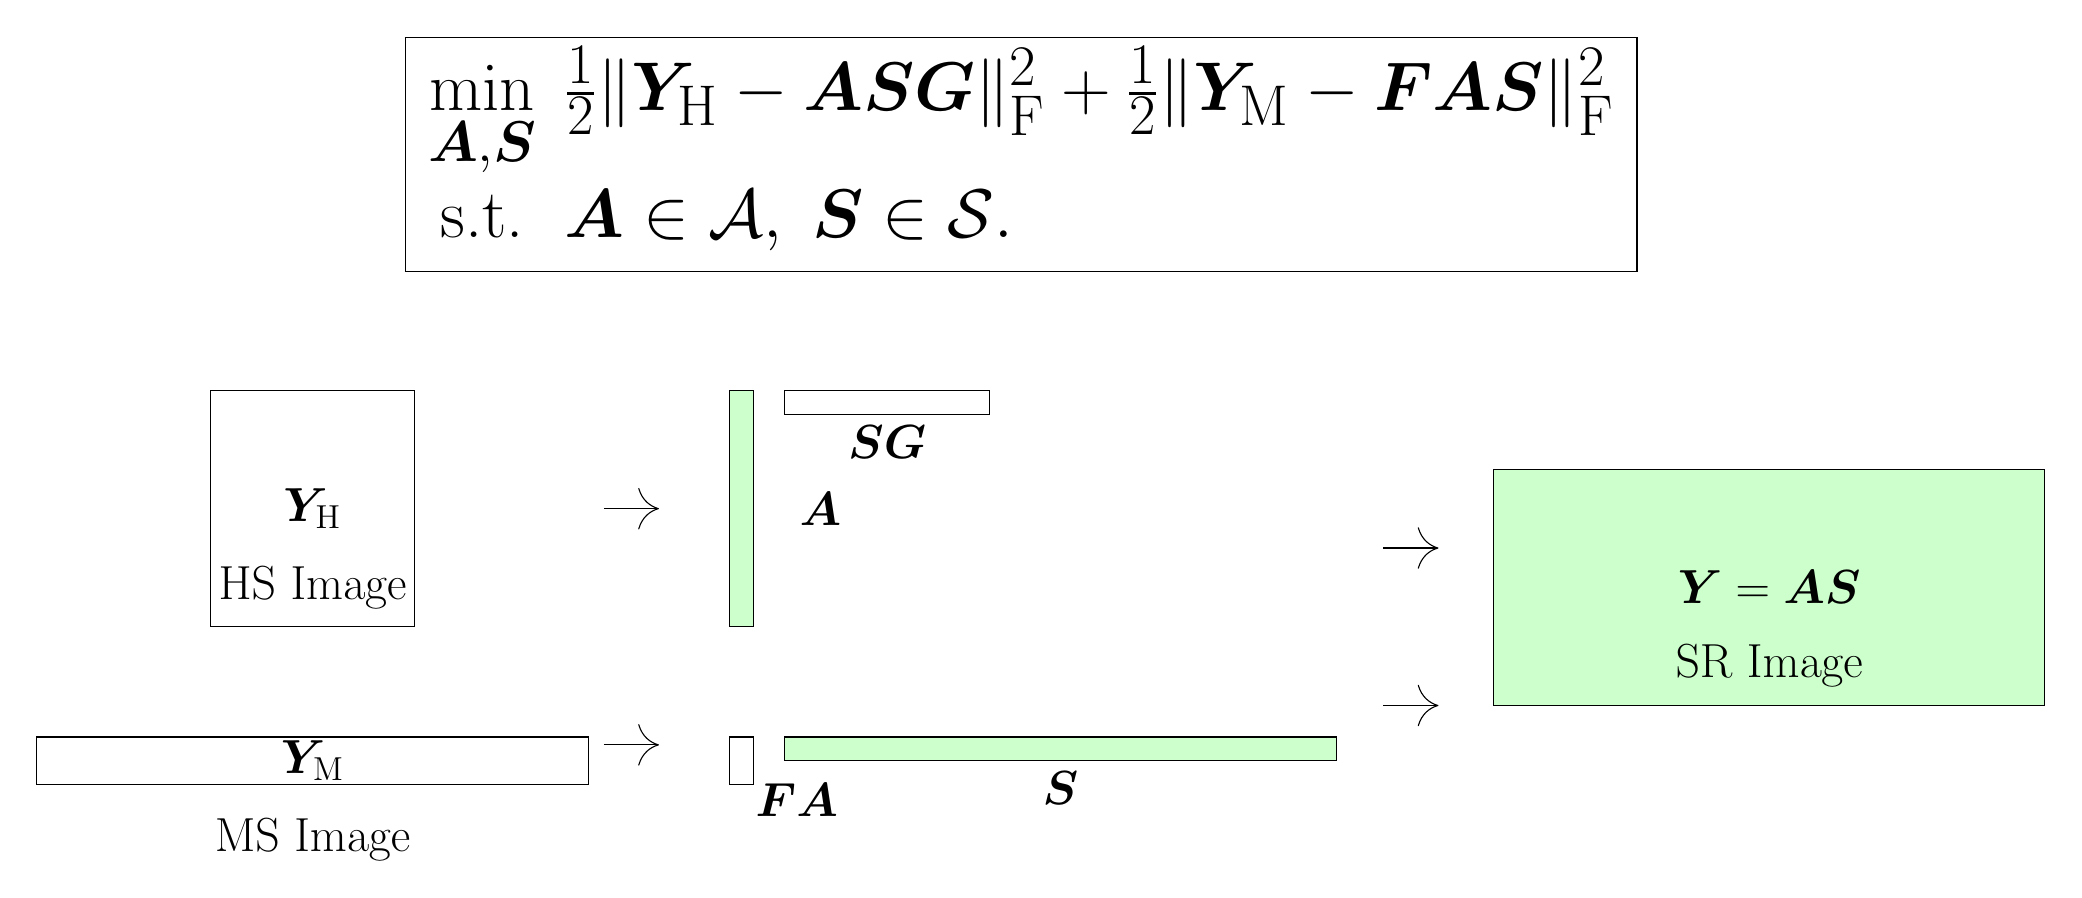
\begin{tikzpicture}
                    \node at (-6,0) (nsource) {$\;$} ;
                    \node at ( 0,0) (nfactor) {$\;$} ;
                    \node at ( 6,0) (nproduc) {$\;$} ;
                    % the problem formulation
                    \node at (nfactor) [xshift=3cm,yshift=8cm]
                    {$\Huge
                      \boxed{
                          \begin{array}{cl}
                              \underset{\bm A,\bm S}{\min}
                              &
                              \frac{1}{2} \Vert \YH - \bm A \bm S \bm G \Vert\Fr^2 +
                              \frac{1}{2} \Vert \YM - \bm F \bm A \bm S \Vert\Fr^2 \\
                              \text{s.t.}
                              &
                              \bm A \in \mathcal A,\;\bm S \in \mathcal S.
                          \end{array}
                      }$};
                    % HS Matrix
                    \node at (nsource) [xshift=-1.3cm,yshift=5cm] (nYH1) {};
                    \node at (nsource) [xshift= 1.3cm,yshift=2cm] (nYH3) {};
                    \draw (nYH1) rectangle (nYH3) ;
                    \node at ($(nYH1)!0.5!(nYH3)$) (nYH) {\LARGE$\YH$} ;
                    \node at ($(nYH1)!0.5!(nYH3)$) [yshift=-1cm] {\LARGE HS Image};
                    % MS Matrix
                    \node at (nsource) [xshift=  -3.5cm,yshift=0.6cm] (nYM1) {};
                    \node at (nsource) [xshift=   3.5cm,yshift=0.0cm] (nYM3) {};
                    \draw (nYM1) rectangle (nYM3) ;
                    \node at ($(nYM1)!0.5!(nYM3)$) (nYH) {\LARGE$\YM$};
                    \node at ($(nYM1)!0.5!(nYM3)$) [yshift=-1cm] {\LARGE MS Image};
                    % HS factor matrix pair
                    \node at (nfactor) [xshift=   0.0cm,yshift=5.0cm] (nSG1) {};
                    \node at (nfactor) [xshift=   2.6cm,yshift=4.7cm] (nSG3) {};
                    \draw               (nSG1) rectangle (nSG3) ;
                    \node at ($(nSG1)!0.5!(nSG3)$) [yshift=-0.5cm] {\LARGE$\bm S \bm G$};
                    \node at (nfactor) [xshift=  -0.7cm,yshift=2.0cm] (nA1)  {};
                    \node at (nfactor) [xshift=  -0.4cm,yshift=5.0cm] (nA3)  {};
                    \draw [fill=green!20] (nA1)  rectangle (nA3)  ;
                    \node at ($(nA1)!0.5!(nA3)$) [xshift= 1cm] {\LARGE$\bm A$};
                    % MS factor matrix pair
                    \node at (nfactor) [xshift=   0.0cm,yshift=0.3cm] (nS1)  {};
                    \node at (nfactor) [xshift=   7.0cm,yshift=0.6cm] (nS3)  {};
                    \draw [fill=green!20] (nS1)  rectangle (nS3)  ;
                    \node at ($(nS1)!0.5!(nS3)$) [yshift=-0.5cm] {\LARGE$\bm S$};
                    \node at (nfactor) [xshift=  -0.7cm,yshift=0.0cm] (nFA1) {};
                    \node at (nfactor) [xshift=  -0.4cm,yshift=0.6cm] (nFA3) {};
                    \draw               (nFA1) rectangle (nFA3) ;
                    \node at ($(nFA1)!0.5!(nFA3)$) [xshift=0.7cm,yshift=-0.5cm] {\LARGE$\bm F \bm A$};
                    % arrow from HS MS pair to factor pair
                    \draw[-{>[scale=2.5,length=3,width=6]}] (-2.3,3.5) -- (-1.6,3.5) ;
                    \draw[-{>[scale=2.5,length=3,width=6]}] (-2.3,0.5) -- (-1.6,0.5) ;
                    % arrow from factor pair to SR product
                    %\draw[-{>[scale=2.5,length=3,width=6]}] (10.6,3.5) -- (11.3,3.0) ;
                    %\draw[-{>[scale=2.5,length=3,width=6]}] (10.6,0.5) -- (11.3,1.0) ;
                    \draw[-{>[scale=2.5,length=3,width=6]}] ( 7.6,3.0) -- ( 8.3,3.0) ;
                    \draw[-{>[scale=2.5,length=3,width=6]}] ( 7.6,1.0) -- ( 8.3,1.0) ;
                    % SR matrix
                    \node at (nproduc) [xshift= 3cm,yshift=4cm] (nY1) {};
                    \node at (nproduc) [xshift=10cm,yshift=1cm] (nY3) {};
                    \draw [fill=green!20] (nY1)  rectangle (nY3)  ;
                    \node at ($(nY1)!0.5!(nY3)$) {\LARGE$\bm Y = \bm A \bm S$};
                    \node at ($(nY1)!0.5!(nY3)$) [yshift=-1cm]{\LARGE SR Image};
                \end{tikzpicture}
            }
            \caption{Estimate SR image from HS and MS image pair.}
            \label{fig:HSR_problem_visualize}
        \end{figure}
    \end{frame}
\subsection{State of the Arts}
    \begin{frame}
        \frametitle{State of the Arts HSR}
        Two state-of-the-art HSR algorithms: find $\hat{\bm Y} = \bm A \bm S$.
        \begin{itemize}
            \item Coupled Nonnegative Matrix Factorization (CNMF) \cite{CNMF}, solves \\
                  \[\boxed{
                       \begin{array}{cl}
                           \underset{\bm A,\bm S}{\min}
                           &
                           \frac{1}{2} \Vert \YH - \bm A \bm S \bm G \Vert\Fr^2 +
                           \frac{1}{2} \Vert \YM - \bm F \bm A \bm S \Vert\Fr^2 \\
                           \text{s.t.}
                           &
                           \bm A \geq \bm 0,\;\bm S \geq \bm 0;
                       \end{array}
                    }\]
            \item Fusion based on spectral UnMIxing (FUMI) \cite{FUMI}, solves \\
                  \[\boxed{
                       \begin{array}{cl}
                           \underset{\bm A,\bm S}{\min}
                           &
                           \frac{1}{2} \Vert \YH - \bm A \bm S \bm G \Vert\Fr^2 +
                           \frac{1}{2} \Vert \YM - \bm F \bm A \bm S \Vert\Fr^2 \\
                           \text{s.t.}
                           &
                           \bm 0 \leq \bm A \leq \bm 1,\;\bm S \geq \bm 0,\;\bm 1\Tr \bm S = \bm 1\Tr.
                       \end{array}
                    }\]
        \end{itemize}
    \end{frame}
    \begin{frame} \label{fr:SOAs}
        \frametitle{State of the Arts HSR}
        CNMF algorithm \cite{CNMF}: find $\hat{\bm Y} = \bm A \bm S$.
        \begin{itemize}
            \item does not strictly solve the HSR problem;
            \item splits HSR problem into two NMF problems,
                  \ie alternatingly solves \newline
                  \[
                   \boxed{
                       \begin{array}{cl}
                           \underset{\bm A,\bm R}{\min}
                           &
                           \Vert \YH - \bm A \bm R \Vert\Fr^2 \\
                           \text{s.t.}
                           &
                           \bm A, \bm R \geq \bm 0
                       \end{array}
                   }
                  \rightleftharpoons
                  \boxed{
                       \begin{array}{cl}
                           \underset{\bm B,\bm S}{\min}
                           &
                           \Vert \YM - \bm B \bm S \Vert\Fr^2 \\
                           \text{s.t.}
                           &
                           \bm B, \bm S \geq \bm 0
                       \end{array}
                   }
                  \]
            \item an alternating optimization (AO) on $2$ different problems.
            \item \textcolor{blue}{pros}: a fast method available: Lee-Seung
                  Multiplicative Update \cite{LSMU_NATURE1999} \hyperlink{fr:LSMU}{\beamergotobutton{\tiny details}}
            \item \textcolor{red}{cons}: a heuristic apprach, no convergence guarantee from
            \item[]\hspace{0.8cm} optimization view point.
        \end{itemize}
    \end{frame}
    \begin{frame}
        \frametitle{State of the Arts HSR}
        FUMI algorithm \cite{FUMI}: find $\hat{\bm Y} = \bm A \bm S$.
        \begin{itemize}
            \item alternatingly solves \newline
        \end{itemize}
        \[\begin{array}{c}
          \boxed{
             \begin{array}{cl}
                 \underset{\bm A}{\min}
                 &
                 \frac{1}{2} \Vert \YH - \bm A \bm S \bm G \Vert\Fr^2
                 +
                 \frac{1}{2} \Vert \YM - \bm F \bm A \bm S \Vert\Fr^2 \\
                 \text{s.t.}
                 &
                 \bm 0 \leq \bm A \leq \bm 1,
             \end{array}
          } \\
          \text{\rotatebox{90}{$\rightleftharpoons$}} \\
          \boxed{
             \begin{array}{cl}
                 \underset{\bm S}{\min}
                 &
                 \frac{1}{2} \Vert \YH - \bm A \bm S \bm G \Vert\Fr^2
                 +
                 \frac{1}{2} \Vert \YM - \bm F \bm A \bm S \Vert\Fr^2 \\
                 \text{s.t.}
                 &
                 \bm S \geq \bm 0, \; \bm 1\Tr \bm S = \bm 1\Tr
             \end{array}
          }
          \end{array}\]
        \begin{itemize}
            \item an AO on the same problem;
            \item uses ADMM to solve;
            \item \textcolor{blue}{pros}: has convergence guarantee.
            %\item \textcolor{red}{cons}: ADMM requires solving matrix inverse problems;
            \item \textcolor{red}{cons}: unsuitable for big matrix problems ($\bm G$ is potentially large);
            \item \textcolor{red}{cons}: highly depends on special structure of $\bm G$.
        \end{itemize}
    \end{frame}
    \begin{frame}
        \frametitle{State of the Arts HSR}
        Some more state of the arts ... \\
        \vspace{1cm}
        Sparse Promoting NMF \cite{SNNMF}:
        \[ \begin{array}{cl}
               \underset{\bm A,\bm S}{\min}
               &
               \frac{1}{2} \Vert \YH - \bm A \bm S \bm G \Vert\Fr^2
               +
               \frac{1}{2} \Vert \YM - \bm F \bm A \bm S \Vert\Fr^2
               \textcolor{red}{\; + \; \lambda \; \text{sparse} (\bm S)} \\
               \text{s.t.}
               &
               \bm A, \; \bm S \geq \bm 0;
           \end{array} \]
        HYperspectral SUper-REsolution (HYSURE) \cite{CONVEX_FORMULATION_HSR_VIA_SUBSPACE_REGULAR}:\\
        with an estimated endmember $\hat{\bm A}$,
        \[ \begin{array}{cl}
               \underset{\bm S}{\min}
               &
               \frac{1}{2} \Vert \YH - \hat{\bm A} \bm S \bm G \Vert\Fr^2
               +
               \frac{1}{2} \Vert \YM - \bm F \hat{\bm A} \bm S \Vert\Fr^2
               \textcolor{red}{\; + \; \lambda \; \text{TV} (\bm S)}.
           \end{array}\]
    \end{frame}
\section{Fast Algorithm Framework of HSR (proposed)}
\subsection{Preliminaries}
    \begin{frame}
        \frametitle{Preliminaries}
        Let $f(\bm A,\bm S)
             = \frac{1}{2} \Vert \YH - \bm A \bm S \bm G \Vert\Fr^2
             + \frac{1}{2} \Vert \YM - \bm F \bm A \bm S \Vert\Fr^2$ and $\mathcal S$, $\mathcal A$ are convex. \\
        \vspace{0.3cm}
        We focus on the basic HSR problem:
        \begin{equation}
            \begin{array}{cl}
                \underset{\bm A,\bm S}{\min}
                &
                f(\bm A,\bm S) \\
                \text{s.t.}
                &
                \bm A \in \mathcal A, \; \bm S \in \mathcal S.
                %\bm 0 \leq \bm A \leq \bm 1, \; \bm S \geq \bm 0, \; \bm 1\Tr \bm S = \bm 1\Tr.
            \end{array}
            \label{eq:HSR}
        \end{equation}
        Traditionally, people use AO to solve \eqref{eq:HSR},
        \ie iterate for $k=0,1,\cdots$
        \begin{eqnarray}
            \bm S\iter{k+1} & \gets & \begin{array}{cl} \underset{\bm S \in \mathcal S}{\min} & f(\bm A\iter{k},\bm S)   \end{array} \label{eq:HSR_S} \\
            \bm A\iter{k+1} & \gets & \begin{array}{cl} \underset{\bm A \in \mathcal A}{\min} & f(\bm A,\bm S\iter{k+1}) \end{array} \label{eq:HSR_A}
        \end{eqnarray}
        Iterating \eqref{eq:HSR_S} and \eqref{eq:HSR_A} can be seen as a $2$-block coordinate descent (BCD).
    \end{frame}
    \begin{frame} \label{fr:HSR-is-QP}
        \frametitle{Preliminaries}
        HSR by BCD on \eqref{eq:HSR_S} and \eqref{eq:HSR_A}: \\
        \begin{itemize}
            \item successive minimization along direction of $\bm S$ and $\bm A$;
            \item $f(\bm A,\bm S)$ is individually quadratic in $\bm A$ or in $\bm S$;
            \item global solutions to \eqref{eq:HSR_S} and \eqref{eq:HSR_A} are available ($\because$ they are QP \hyperlink{fr:HSR-as-QP}{\beamergotobutton{\tiny details}}).
        \end{itemize}
        \vspace{0.3cm}
        \textcolor{blue}{Pros}:
        \begin{itemize}
            \item can exactly solve for global solutions
                  \textcolor{red}{\textit{if (2),(3) are small}};
            \item can employ ADMM, gradient methods or higher order methods \newline
                  (e.g. Newton's method, interior point methods)
                  \textcolor{red}{\textit{if (2),(3) are small}}.
        \end{itemize}
        \vspace{0.3cm}
        \textcolor{red}{Cons}:
        \begin{itemize}
            \item big data era, interested in big spectral image processing;
            \item \textbf{hard} to exactly solve for global solutions \textcolor{red}{\textit{when (2), (3) are big}};
            \item higher order methods are \textbf{unsuitable} \textcolor{red}{\textit{when (2), (3) are big}}.
        \end{itemize}
    \end{frame}
\subsection{A Very Fast Algorithm Framework}
    \begin{frame}
        \frametitle{Fast Framework of HSR (proposed)}
        Fast framework:
        \begin{itemize}
            \item HSR problem as AO on two QPs, solved by \textcolor{red}{\textit{Inexact}} BCD;
            \item uses $1^{st}$ order gradient methods, which can be
                  \begin{itemize}
                      \item Gradient Projection (GP) type methods:
                            \begin{itemize}
                                \item GP \cite{NONLINEAR_PRGM},
                                \item Barzilai-Borwein GP (BBGP) \cite{BARZILAI_BORWEIN_ALGORITHM};
                            \end{itemize}
                      \item Proximal Gradient (PG) type methods:
                            \begin{itemize}
                                \item PG \cite{PROX_ALGO},
                                \item Fast PG (FISTA) \cite{NESTEROV_FISTA,A_FAST_ITERA_SHRINK_THRESH_ALGO};
                            \end{itemize}
                      \item Projection-free type method:
                            \begin{itemize}
                                \item Frank-Wolfe (FW) \cite{FRANKWOLFE_AN_ALGO_FOR_QUAD_PRGM}.
                            \end{itemize}
                  \end{itemize}
            %\item $1^{st}$ order gradient methods
            %      \begin{itemize}
            %          \item all require gradient computation;
            %          \item except FW, all require projection onto constraint set.
            %      \end{itemize}
        \end{itemize}
    \end{frame}
    \begin{frame}
        \frametitle{Fast Framework of HSR (proposed)}
        A brief overview on $1^{st}$ order gradient methods. \\
        Suppose $g(\bm x)$ is quadratic in $\bm x$, and $\mathcal X$ is the
        feasible set of $\bm x$. \\
        We repeat, for $k = 0,1,\cdots$,
        \begin{equation}
            \begin{array}{c}
                \bm x\iter{k+1} \gets \bm x\iter{k} + \gamma\iter{k} \bm d\iter{k}, \\
                \text{\footnotesize  (GP, BBGP and FW, with $\bm d\iter{k} \in \mathcal X$)}
            \end{array}
            \label{eq:FOGM_Upd_GPFW}
        \end{equation}
        or
        \begin{equation}
            \begin{array}{c}
                \bm x\iter{k+1} \gets \Pi_{\mathcal X}\left( \bm x\iter{k} + \gamma\iter{k} \bm d\iter{k} \right). \\
                \text{\footnotesize  (PG and FISTA, with $\bm d\iter{k} \in \text{or} \notin \mathcal X$)}
            \end{array}
            \label{eq:FOGM_Upd_PG}
        \end{equation}
        \begin{itemize}
            \item $\bm d\iter{k}$ is the descent direction,
                  can be the direction opposite to $\nabla g(\bm x\iter{k})$,
                  or any directions that guarantee $g(\bm x\iter{k+1}) \leq g(\bm x\iter{k})$;
            \item $\gamma\iter{k}$ is the step size;
        \end{itemize}
    \end{frame}
    \begin{frame}
        \frametitle{Fast Framework of HSR (proposed)}
        A brief overview on $1^{st}$ order gradient methods.
        \begin{table}
            \begin{tabular}{c|ccccc}
                $1^{st}$ order method                            & GP                         & BBGP                       & PG                         & FISTA                      & FW                         \tabularnewline \hline
                requires $\nabla g(\bm x\iter{k})$ computation   & \textcolor{blue}\checkmark & \textcolor{blue}\checkmark & \textcolor{blue}\checkmark & \textcolor{blue}\checkmark & \textcolor{blue}\checkmark \tabularnewline
                requires projection in finding $\bm d\iter{k}$   & \textcolor{blue}\checkmark & \textcolor{blue}\checkmark & \textcolor{red}{\textit{X}}& \textcolor{red}{\textit{X}}& \textcolor{red}{\textit{X}}\tabularnewline
                requires projection in finding $\bm x\iter{k+1}$ & \textcolor{red}{\textit{X}}& \textcolor{red}{\textit{X}}& \textcolor{blue}\checkmark & \textcolor{blue}\checkmark & \textcolor{red}{\textit{X}}\tabularnewline
                requires searching for $\gamma\iter{k}$          & \textcolor{blue}\checkmark & \textcolor{blue}\checkmark & \textcolor{red}{\textit{X}}& \textcolor{red}{\textit{X}}& \textcolor{blue}\checkmark
            \end{tabular}
        \end{table}
    \end{frame}
    \begin{frame}
        \frametitle{Fast Framework of HSR (proposed)}
        Traditionally, people do the following:
        \begin{algorithm}[H]
            \caption{HSR by Exact BCD with $1^{st}$ order gradient methods}
            \begin{algorithmic}[1]
                \Procedure{}{} 
                \newline
                Input: %$\YH$,
                       %$\YM$,
                       %$\bm F$,
                       %$\bm G$,
                       $\bm S\iter{0}\in\mathcal S$,
                       $\bm A\iter{0}\in\mathcal A$; \;\;\;
                Output: $\bm A\iter{K+1}$, $\bm S\iter{K+1}$.
                \smallskip
                \For{$k=0,1,2,\cdots,K$}% until stopping criteria holds}
                    \color{red}
                    \For{$j=1,2,\cdots,J$}% or until stopping criteria holds}
                        \State{$\bm S\iter{k} \gets
                                \texttt{1st\_GradUpd}%_{\bm s}
                                (f(\bm A\iter{k},\bm S\iter{k}))$.}
                    \EndFor
                    \State{$\bm S\iter{k+1} \gets \bm S\iter{k}$.}
                    \color{blue}
                    \For{$j=1,2,\cdots,J$}% or until stopping criteria holds}
                        \State{$\bm A\iter{k} \gets
                                \texttt{1st\_GradUpd}%_{\bm a}
                                (f(\bm A\iter{k},\bm S\iter{k+1}))$.}
                    \EndFor
                    \State{$\bm A\iter{k+1} \gets \bm A\iter{k}$.}
                    \color{black}
                \EndFor
            \EndProcedure
            \end{algorithmic}
            \label{alg:GEN_FRAMEWORK_OF_HSR_BY_FOGM_EXACT_BCD}
        \end{algorithm}
    \end{frame}
    \begin{frame}
        \frametitle{Fast Framework of HSR (proposed)}
        The proposed fast framework does the following:
        HSR by Inexact BCD with $1^{st}$ order methods (named
        \textcolor{orange}{AL}ternating \textcolor{orange}{G}radient-based
        \textcolor{orange}{O}ptimization \textcolor{orange}{ALGO})
        \begin{algorithm}[H]
            \caption{HSR by ALGO}
            \begin{algorithmic}[1]
                \Procedure{}{} 
                \newline
                Input: %$\YH$,
                       %$\YM$,
                       %$\bm F$,
                       %$\bm G$,
                       $\bm S\iter{0}\in\mathcal S$,
                       $\bm A\iter{0}\in\mathcal A$; \;\;\;
                Output: $\bm A\iter{K+1}$, $\bm S\iter{K+1}$.
                \smallskip
                \For{$k=0,1,2,\cdots,K$}% until stopping criteria holds}
                    \color{red}
                        \State{$\bm S\iter{k+1} \gets
                                \texttt{1st\_GradUpd}%_{\bm s}
                                (f(\bm A\iter{k},\bm S\iter{k}))$.}
                    \color{blue}
                        \State{$\bm A\iter{k+1} \gets
                                \texttt{1st\_GradUpd}%_{\bm a}
                                (f(\bm A\iter{k},\bm S\iter{k+1}))$.}
                    \color{black}
                \EndFor
            \EndProcedure
            \end{algorithmic}
            \label{alg:GEN_FRAMEWORK_OF_HSR_BY_FOGM_INEXACT_BCD}
        \end{algorithm}
    \end{frame}
    \begin{frame}
        \frametitle{Fast Framework of HSR (proposed)}
        \begin{algorithm}[H]
            \caption*{HSR by ALGO}
            \begin{algorithmic}[1]
                \Procedure{}{} 
                \newline
                Input: %$\YH$,
                       %$\YM$,
                       %$\bm F$,
                       %$\bm G$,
                       $\bm S\iter{0}\in\mathcal S$,
                       $\bm A\iter{0}\in\mathcal A$; \;\;\;
                Output: $\bm A\iter{K+1}$, $\bm S\iter{K+1}$.
                \smallskip
                \For{$k=0,1,2,\cdots,K$}% until stopping criteria holds}
                    \color{red}
                        \State{$\bm S\iter{k+1} \gets
                                \texttt{1st\_GradUpd}%_{\bm s}
                                (f(\bm A\iter{k},\bm S\iter{k}))$.}
                    \color{blue}
                        \State{$\bm A\iter{k+1} \gets
                                \texttt{1st\_GradUpd}%_{\bm a}
                                (f(\bm A\iter{k},\bm S\iter{k+1}))$.}
                    \color{black}
                \EndFor
            \EndProcedure
            \end{algorithmic}
        \end{algorithm}
        Remark:
        \begin{itemize}
            \item special case of Algorithm 1 when $J = 1$;
            \item \texttt{1st\_GradUpd} is a \textbf{one-step} gradient
                  update either in \eqref{eq:FOGM_Upd_GPFW} or \eqref{eq:FOGM_Upd_PG};
            %\item inexact update of variables; % yet the objective is sure to be decreased
            \item in $1$ outer iteration, \textcolor{orange}{ALGO} is
                  \textbf{much faster} than Exact BCD.
        \end{itemize}
    \end{frame}
    \begin{frame}
        \frametitle{Fast Framework of HSR (proposed)}
        \begin{algorithm}[H]
            \caption*{HSR by ALGO}
            \begin{algorithmic}[1]
                \Procedure{}{} 
                \newline
                Input: %$\YH$,
                       %$\YM$,
                       %$\bm F$,
                       %$\bm G$,
                       $\bm S\iter{0}\in\mathcal S$,
                       $\bm A\iter{0}\in\mathcal A$; \;\;\;
                Output: $\bm A\iter{K+1}$, $\bm S\iter{K+1}$.
                \smallskip
                \For{$k=0,1,2,\cdots,K$}% until stopping criteria holds}
                    \color{red}
                        \State{$\bm S\iter{k+1} \gets
                                \texttt{1st\_GradUpd}%_{\bm s}
                                (f(\bm A\iter{k},\bm S\iter{k}))$.}
                    \color{blue}
                        \State{$\bm A\iter{k+1} \gets
                                \texttt{1st\_GradUpd}%_{\bm a}
                                (f(\bm A\iter{k},\bm S\iter{k+1}))$.}
                    \color{black}
                \EndFor
            \EndProcedure
            \end{algorithmic}
        \end{algorithm}
        Remark:
        \begin{itemize}
            \item with $f(\bm A,\bm S)
                        = \frac{1}{2}\Vert \YH - \bm{ASG} \Vert\Fr^2
                        + \frac{1}{2}\Vert \YM - \bm{FAS} \Vert\Fr^2$,\newline
                  gradient is just some algebrae:
                  \begin{itemize}
                      \item \textcolor{red}{
                            $\nabla_{\bm S} f(\bm A,\bm S)
                             = \bm A\Tr\bm{ASGG}\Tr + (\bm{FA})\Tr\bm{FAS}
                             - \bm A\Tr\YH\bm G\Tr  - (\bm{FA})\Tr\YM$},
                      \item \textcolor{blue}{
                            $\nabla_{\bm A} f(\bm A,\bm S)
                             = \bm{ASG}(\bm{SG})\Tr + \bm F\Tr\bm{FASS}\Tr
                             - \YH(\bm{SG})\Tr      - \bm F\Tr\YM\bm S\Tr$}.
                  \end{itemize}
        \end{itemize}
    \end{frame}
    \begin{frame}
        \frametitle{Fast Framework of HSR (proposed)}
        \begin{algorithm}[H]
            \caption*{HSR by ALGO}
            \begin{algorithmic}[1]
                \Procedure{}{} 
                \newline
                Input: %$\YH$,
                       %$\YM$,
                       %$\bm F$,
                       %$\bm G$,
                       $\bm S\iter{0}\in\mathcal S$,
                       $\bm A\iter{0}\in\mathcal A$; \;\;\;
                Output: $\bm A\iter{K+1}$, $\bm S\iter{K+1}$.
                \smallskip
                \For{$k=0,1,2,\cdots,K$}% until stopping criteria holds}
                    \color{red}
                        \State{$\bm S\iter{k+1} \gets
                                \texttt{1st\_GradUpd}%_{\bm s}
                                (f(\bm A\iter{k},\bm S\iter{k}))$.}
                    \color{blue}
                        \State{$\bm A\iter{k+1} \gets
                                \texttt{1st\_GradUpd}%_{\bm a}
                                (f(\bm A\iter{k},\bm S\iter{k+1}))$.}
                    \color{black}
                \EndFor
            \EndProcedure
            \end{algorithmic}
        \end{algorithm}
        Remark:
        \begin{itemize}
            \item \texttt{1st\_GradUpd()} can be chosen as one of the following:
                  \begin{itemize}
                      \item Grad. Proj. type: \texttt{GP\_Upd()}, \texttt{BBGP\_Upd()};
                      \item Prox. Grad. type: \texttt{PG\_Upd()}, \texttt{FISTA\_Upd()};
                      \item Proj. Free type: \texttt{FW\_Upd()}.
                  \end{itemize}
        \end{itemize}
    \end{frame}
\section{Experiments}
    \begin{frame}
        \frametitle{Experiments}
        HSR experimental objectives: to see
        \begin{itemize}
            \item [1)] if we use $1^{st}$ order gradient algorithms, which one is better ? \\
                       Exact BCD or \textcolor{orange}{ALGO} ?
            \item [2)] comparing with CNMF \& FUMI, can traditional BCD or
                       \textcolor{orange}{ALGO} have better performance ?
        \end{itemize}
        \vspace{0.5cm}
        Performance measure:
        \begin{itemize}
            \item global measure:   {\footnotesize $\displaystyle \text{RMSE}(\bm Y,\hat{\bm Y}) \coloneqq \frac{\Vert \bm Y - \hat{\bm Y} \Vert\Fr}{\sqrt{ML}}$};
                  \begin{itemize}
                      \item [] $\rightarrow$ lower the better
                  \end{itemize}
            \item spectral measure: {\footnotesize $\displaystyle \text{SAM}(\bm Y,\hat{\bm Y}) \coloneqq \frac{1}{L} \sum_{j=1}^L \cos\inv\left( \frac{\langle \bm y[\;j\;] \;,\; \hat{\bm y}[\;j\;] \rangle}{\Vert \bm y[\;j\;] \Vert_2 \;\; \Vert \hat{\bm y}[\;j\;] \Vert_2} \right)$};
                  \begin{itemize}
                      \item [] $\rightarrow$ lower the better
                  \end{itemize}
            \item spatial measure:  {\footnotesize $\displaystyle \text{PSNR}(\bm Y,\hat{\bm Y}) \coloneqq \frac{1}{M} \sum_{i=1}^M 10 \log_{10} \left( \frac{\max(\bm y^i)}{\Vert \bm y^i - \hat{\bm y}^i \Vert_2^2 / L} \right)$}.
                  \begin{itemize}
                      \item [] $\rightarrow$ higher the better
                  \end{itemize}
        \end{itemize}
    \end{frame}
    \begin{frame}
        \frametitle{Experiments}
        Testing subjects: \\
        from $2$ real spectral image data sets: "Chikusei" \cite{NYOKOYA2016} and "Cuprite" \cite{AVIRIS}.
        \begin{figure}
            \resizebox{0.9\linewidth}{!}{
            \begin{tikzpicture}
                \node at (0,0) (nCenter) {};
                \node at (nCenter) [xshift=-2.7cm] (nChik) {\includegraphics[width=0.48\linewidth]{./figures/chikusei_RGB}};%chikusei_1000x1000_815nm_normalized}} ;
                \node at (nCenter) [xshift= 2.7cm] (nCupr) {\includegraphics[width=0.48\linewidth]{./figures/cuprite_RGB}             };%cuprite_200x348_815nm_normalized}} ;
                \node at (nChik)   [yshift=-3.2cm,text width=4.5cm] {\small (a) Chikusei data set, with $128$ spectral bands, $1000^2$ pixels.};
                \node at (nCupr)   [yshift=-3.2cm,text width=4.5cm] {\small (b) Cuprite data set, with $224$ spectral bands, $200\times348$ pixels.};
            \end{tikzpicture}
            }
            \caption{Color image of Chikusei and Cuprite data set.}
        \end{figure}
    \end{frame}
    \begin{frame}
        \frametitle{Experiments}
        Experimental flow and data preparation.
        \begin{figure}
            \centering
            \resizebox{0.90\linewidth}{!}{
                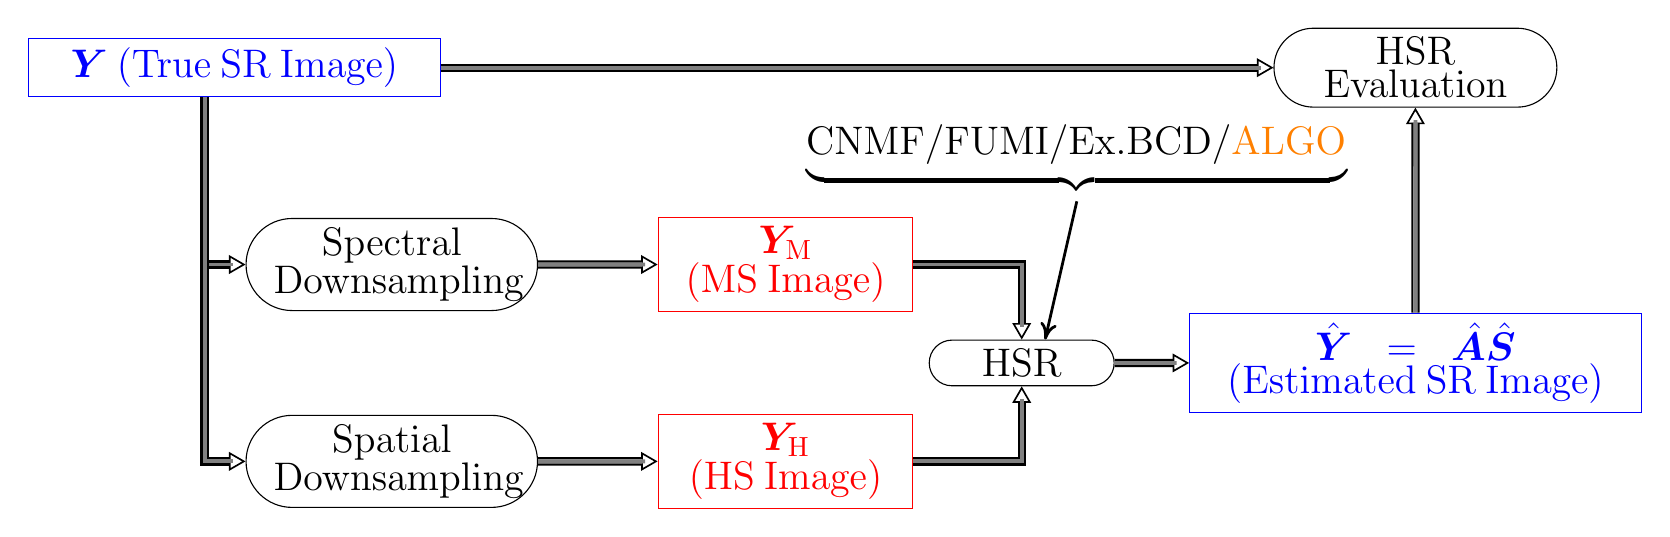
\begin{tikzpicture}
                    \node at (0,0)               [xshift=   0cm,yshift=   0cm,draw                  ,text width=5.0cm,align=center, blue!100] (nSR)  {\Large $\bm Y$ (True SR Image)};
                    \node at (nSR)               [xshift= 2.0cm,yshift=-2.5cm,draw,rounded rectangle,text width=3.0cm,align=center,black!100] (nF)   {\Large Spectral\\Downsampling};
                    \node at (nSR)               [xshift= 2.0cm,yshift=  -5cm,draw,rounded rectangle,text width=3.0cm,align=center,black!100] (nG)   {\Large Spatial\\Downsampling};
                    \node at (nF)                [xshift=   5cm,yshift=   0cm,draw                  ,text width=3.0cm,align=center,  red!100] (nMS)  {\Large $\YM$\\(MS Image)};
                    \node at (nG)                [xshift=   5cm,yshift=   0cm,draw                  ,text width=3.0cm,align=center,  red!100] (nHS)  {\Large $\YH$\\(HS Image)};
                    \node at ($(nHS)!0.5!(nMS)$) [xshift=   3cm,yshift=   0cm,draw,rounded rectangle,text width=2.0cm,align=center,black!100] (nHSR) {\Large HSR};
                    \node at (nHSR)              [xshift= 5.0cm,yshift=   0cm,draw                  ,text width=5.5cm,align=center, blue!100] (nSR2) {\Large $\hat{\bm Y}=\hat{\bm A}\hat{\bm S}$\\(Estimated SR Image)};
                    \node at (nSR2)              [xshift=   0cm,yshift=3.75cm,draw,rounded rectangle,text width=3.0cm,align=center,black!100] (nEva) {\Large HSR\\ Evaluation};
                    \draw[vecArrow] (nSR.-135) |- (nF)       ;
                    \draw[vecArrow] (nSR.-135) |- (nG)       ;
                    \draw[vecArrow] (nF.0)     to (nMS.180)  ;
                    \draw[vecArrow] (nG.0)     to (nHS.180)  ;
                    \draw[vecArrow] (nMS.0)    -| (nHSR)     ;
                    \draw[vecArrow] (nHS.0)    -| (nHSR)     ;
                    \draw[vecArrow] (nHSR.0)   to (nSR2.180) ;
                    \draw[vecArrow] (nSR.0)    to (nEva.180) ;
                    \draw[vecArrow] (nSR2.90)  to (nEva.-90) ;
                    \node at (nHSR) [xshift=0.7cm,yshift=2.6cm] (nMethods) {\Large $\underbrace{\text{CNMF/FUMI/Ex.BCD/\color{orange}ALGO}_{}}$} ;
                    \draw[-{>[scale=1.5,length=4,width=4]},line width=1.0] (nMethods.-90) -- (nHSR.45);
                \end{tikzpicture}
            }
            \caption{Wald's Protocol \cite{WALDS_PROTOCOL} on HS and MS images synthesis and the evaluation
                     of a testing HSR method.}
            \label{fig:Walds_Protocol}
        \end{figure}
    \end{frame}
    \begin{frame}
        \frametitle{Experiments}
        Experimental setup:
        \begin{itemize}
            \item use real hyperspectral images as the super-resolution (SR) image;
                  \begin{itemize}
                      \item over $100$ spectral bands from $0.4\,\mu$m to $3\,\mu$m wavelength.
                  \end{itemize}
            \item generate HS image from the SR image by
                  \begin{itemize}
                      \item passing through a Gaussian filter, $2$-D mask: $11 \times 11$, $\sigma = 1.7$;
                      \item subsampling on every $4$ pixels in vertical and horizontal directions.
                  \end{itemize}
        \end{itemize}
        \begin{figure}
            \centering
            \resizebox{0.98\linewidth}{!}{
            \begin{tikzpicture}
                \node at (nCenter)                 (nFull)          {\includegraphics[width=0.25\linewidth]{./figures/IMG_DOWNSAMP_full400x400}};
                \node at (nFull)  [xshift= 4.5 cm] (nBlur)          {\includegraphics[width=0.25\linewidth]{./figures/IMG_DOWNSAMP_blur400x400}};
                \node at (nBlur)  [xshift= 3.5 cm] (nDown)          {\includegraphics[width=0.08\linewidth]{./figures/IMG_DOWNSAMP_down50x50}  };
                \node at (nFull)  [yshift=-2.0 cm] {SR image};
                \node at (nBlur)  [yshift=-2.0 cm] {Blurred SR image};
                \node at (nDown)  [yshift=-2.0 cm] {HS image};
                \draw[-{>[scale=1.5,length=4,width=4]},line width=1.0] (nFull.0) -- (nBlur.180);
                \draw[-{>[scale=1.5,length=4,width=4]},line width=1.0] (nBlur.0) -- (nDown.180);
                \node at ($(nFull)!0.5!(nBlur)$) [yshift=0.6cm] {\footnotesize low-pass filter};
                \node at ($(nBlur)!0.5!(nDown)$) [xshift=0.5cm,yshift=0.6cm] {\footnotesize subsample};
            \end{tikzpicture}
            }
            \caption{From SR image to HS image, visualized by RGB component.}
        \end{figure}
    \end{frame}
    \begin{frame}
        \frametitle{Experiments}
        Experimental setup:
        \begin{itemize}
            %\item use real hyperspectral images as the super-resolution (SR) image;
            %      \begin{itemize}
            %          \item over $100$ spectral bands from $0.4\,\mu$m to $3.9\,\mu$m wavelength.
            %      \end{itemize}
            \item generate MS image from real SR image by
                  \begin{itemize}
                      \item simulate each band of MS band image by taking the
                            average of all band image within the respective passed-band. \newline
                  \end{itemize}
        \end{itemize}
        \begin{figure}
            \resizebox{0.95\linewidth}{!}{
            \begin{tikzpicture}
            \node at (0,0) (ntable) {\begin{tabular}{|c|l|}
                                         \hline
                                         Wavelength ($\mu$m)              & Spectral Band Placement                          \\ \hline
                                         \textcolor{blue}  {$0.45 - 0.52$}& \textcolor{blue}  {Visible (VIS-B)             } \\
                                         \textcolor{olive} {$0.52 - 0.60$}& \textcolor{olive} {Visible (VIS-G)             } \\
                                         \textcolor{red}   {$0.63 - 0.69$}& \textcolor{red}   {Visible (VIS-R)             } \\
                                         \textcolor{purple}{$0.76 - 0.90$}& \textcolor{purple}{Near Infrared (NIR)         } \\ \hline
                                         %\textcolor{cyan}  {$1.55 - 1.75$}& \textcolor{cyan}  {Short Wave Infrared (SWIR-1)} \\
                                         %\textcolor{brown} {$2.08 - 2.35$}& \textcolor{brown} {Short Wave Infrared (SWIR-2)} \\ \hline
                                     \end{tabular}
                                    };
            \node at (ntable) [xshift=-6.5cm] (nHSI) {\includegraphics[width=3cm]{./figures/HSI}};
            \node at (ntable) [xshift= 6.5cm] (nMS)  {\includegraphics[width=1.8cm]{./figures/MS_4bands}};
            \node at (nHSI)   [yshift=-1.8cm]        {SR image};
            \node at (nMS)    [yshift=-1.8cm]        {MS image};
            \node at (ntable) [yshift=-3.8cm] (nHSMS-relation) {\includegraphics[width=1.2\linewidth]{./figures/HSMS_response_AVIRIS_LANDSAT}};
            \node at (ntable) [yshift=-1.8cm] {(a) Pass bands of TM sensor in LANDSA 7 Project};
            \draw[-{>[scale=1.5,length=4,width=4]},line width=1.0] (nHSI.0) -- (ntable.180);
            \draw[-{>[scale=1.5,length=4,width=4]},line width=1.0] (ntable.0) -- (nMS.180);
            \node at (nHSMS-relation) [yshift=-1.8cm] {(b) Center wavelengths of HS bands (\textcolor{blue}{blue bars})
                                                           and spectral response of TM sensor (\textcolor{red}{red}).};
            \end{tikzpicture}
            }
        \end{figure}
    \end{frame}
    \begin{frame}
        \frametitle{Experiments}
        Part I: Exact BCD vs \textcolor{orange}{ALGO} on Cuprite data set. \\
        Implementing Algorithm \ref{alg:GEN_FRAMEWORK_OF_HSR_BY_FOGM_EXACT_BCD}
        by adjusting $J = \begin{cases}
                              100, & \text{Exact BCD}; \\
                              1,   & {\color{orange}\text{ALGO}}.
                          \end{cases}$
        \begin{table}
            \centering
            \resizebox{0.98\linewidth}{!}{
            \begin{tabular}{|c|c|c|c|c|c|c|}
            \hline
            %\multicolumn{ 6}{|c|}{$N = 16$} \tabularnewline \hline
            SNR (dB)            & Method        & RMSE(dB)                             & SAM(deg.)                          & PSNR(dB)                            & Outer Iter.           \tabularnewline \hline
            %--------------------------------------------------------------------------------------------------------------------------------------------------------------------------------------------------%
            \multirow{2}{*}{40} & ALGO-GP       & \cellcolor{red!10}{$-23.18\pm 0.08$} & \cellcolor{red!10}{$0.88\pm 0.01$} & \cellcolor{red!10}{$44.27\pm 0.13$} & $984.38   \pm 50.37$  \tabularnewline
                                & Ex.BCD-GP     &                   {$-21.78\pm 0.16$} &                   {$1.19\pm 0.03$} &                   {$42.06\pm 0.22$} & $243.32   \pm 14.47$  \tabularnewline \hline
            \multirow{2}{*}{20} & ALGO-GP       & \cellcolor{red!10}{$-16.01\pm 0.04$} & \cellcolor{red!10}{$4.27\pm 0.05$} & \cellcolor{red!10}{$28.77\pm 0.09$} & $195.02   \pm 10.27$  \tabularnewline
                                & Ex.BCD-GP     &                   {$-14.27\pm 0.13$} &                   {$6.87\pm 0.25$} &                   {$25.28\pm 0.26$} & $54.99    \pm 4.19$   \tabularnewline \hline
            %--------------------------------------------------------------------------------------------------------------------------------------------------------------------------------------------------%
            \end{tabular}
            }
            \caption{HSR performance of \textcolor{orange}{ALGO-GP} and
                     Ex.BCD-GP on Cuprite dataset.}
        \end{table}
        \begin{table}
            \centering
            \resizebox{0.98\linewidth}{!}{
            \begin{tabular}{|c|c|c|c|c|c|c|}
            \hline
            %\multicolumn{ 6}{|c|}{$N = 16$} \tabularnewline \hline
            SNR (dB)            & Method        & RMSE(dB)                             & SAM(deg.)                          & PSNR(dB)                            & Outer Iter.           \tabularnewline \hline
            %--------------------------------------------------------------------------------------------------------------------------------------------------------------------------------------------------%
            \multirow{2}{*}{40} & ALGO-PG       & \cellcolor{red!10}{$-23.38\pm 0.02$} & \cellcolor{red!10}{$0.84\pm 0$}    & \cellcolor{red!10}{$44.77\pm 0.04$} & $2516.63  \pm 98.48$  \tabularnewline
                                & Ex.BCD-PG     &                   {$-23.06\pm 0.06$} &                   {$0.91\pm 0.01$} &                   {$44.08\pm 0.1$}  & $269.25   \pm 20.68$  \tabularnewline \hline
            \multirow{2}{*}{20} & ALGO-PG       & \cellcolor{red!10}{$-16.51\pm 0.02$} & \cellcolor{red!10}{$3.66\pm 0.02$} & \cellcolor{red!10}{$29.88\pm 0.05$} & $475.63   \pm 25.43$  \tabularnewline
                                & Ex.BCD-PG     &                   {$-15.51\pm 0.04$} &                   {$4.95\pm 0.05$} &                   {$27.72\pm 0.09$} & $80.46    \pm 4.28$   \tabularnewline \hline
            %--------------------------------------------------------------------------------------------------------------------------------------------------------------------------------------------------%
            \end{tabular}
            }
            \caption{HSR performance of \textcolor{orange}{ALGO-PG} and
                     Ex.BCD-PG on Cuprite dataset.}
        \end{table}
    \end{frame}
    \begin{frame}
        \frametitle{Experiments}
        Part 1: Exact BCD vs \textcolor{orange}{ALGO} on Cuprite data set.
        \begin{figure}
            \resizebox{0.88\linewidth}{!}{
            \begin{tikzpicture}
                \node at (0,0) (nCenter) {} ;
                \node at (nCenter)                   (nRGB)          {\includegraphics[width=0.42\linewidth]{./figures/cuprite_RGB}} ;
                \node at (nRGB)     [xshift= 5.0 cm] (nALGO-GP)      {\includegraphics[width=0.42\linewidth]{./figures/SAM_MAP_ALGO-GP}} ;
                \node at (nRGB)     [yshift=-3.5 cm] (nHisto)        {\includegraphics[width=0.55\linewidth]{./figures/ALGO-GP_vs_ExBCD-GP_SAMmap}} ;
                \node at (nALGO-GP) [yshift=-3.5 cm] (nExBCD-GP)     {\includegraphics[width=0.42\linewidth]{./figures/SAM_MAP_ExBCD-GP}} ;
                \node at (nRGB)     [yshift=-1.8 cm]                 {\footnotesize (a) RGB image} ;
                \node at (nALGO-GP) [yshift=-1.8 cm]                 {\footnotesize (b) SAM map of \textcolor{orange}{ALGO-GP}} ;
                \node at (nExBCD-GP)[yshift=-1.8 cm]                 {\footnotesize (c) SAM map of Ex.BCD-GP} ;
                \node at (nHisto)   [yshift=-1.5 cm,text width=5.5cm]{\footnotesize (d) SAM historgram. \textcolor{blue}{Blue}: ALGO-GP; \textcolor{red}{Red}: Ex.BCD-GP.} ;
                \node at ($(nALGO-GP)!0.5!(nExBCD-GP)$) [xshift= 3.0cm]{\includegraphics[width=0.07\linewidth]{./figures/SAM_bar}} ;
            \end{tikzpicture}
            }
            \caption{HSR performance of \textcolor{orange}{ALGO-GP} and Ex.BCD-GP on Cuprite data set.
                     SNR = $40$dB; $N = 16$; $100$ trials.}
        \end{figure}
    \end{frame}
    \begin{frame}
        \frametitle{Experiments}
        Part 1: Exact BCD vs \textcolor{orange}{ALGO} on Synthetic data.
        \begin{table}[h]
        \centering
        \begin{adjustbox}{max width=\textwidth}
        \begin{tabular}{|c|l|c|c|c|c|c|}
        \hline
        SNR (dB)            & \multicolumn{1}{c|}{Method}& RMSE(dB)                              & SAM(deg.)                             & PSNR(dB)                              & Time(sec.)                              & Outer Iter.           \tabularnewline \hline
        %---------------------------------------------------------------------------------------------------------------------------------------------------------------------------------------------------------------------------------------------------------------%
        \multirow{2}{*}{40} & ALGO-GP                    & \cellcolor{red!10}$-15.82   \pm 0.38$ & \cellcolor{red!10}$4.22     \pm 0.4$  & \cellcolor{red!10}$28.9     \pm 0.56$ & \cellcolor{red!10}$13.5     \pm 5.85$   & $878.83   \pm 133.88$ \tabularnewline
                            & Ex.BCD-GP                  &                   $-15.72   \pm 0.4$  &                   $4.37     \pm 0.36$ &                   $28.19    \pm 0.53$ &                   $246.94   \pm 74.52$  & $159.92   \pm 24.28$  \tabularnewline \hline
        %---------------------------------------------------------------------------------------------------------------------------------------------------------------------------------------------------------------------------------------------------------------%
        \multirow{2}{*}{20} & ALGO-GP                    & \cellcolor{red!10}$-14.43   \pm 0.36$ & \cellcolor{red!10}$6.64     \pm 0.28$ & \cellcolor{red!10}$22.66    \pm 0.46$ & \cellcolor{red!10}$3.22     \pm 1.55$   & $178.06   \pm 17.08$  \tabularnewline
                            & Ex.BCD-GP                  &                   $-13.13   \pm 0.44$ &                   $9.84     \pm 0.22$ &                   $20.05    \pm 0.6$  &                   $78.48    \pm 18.32$  & $50.04    \pm 5.78$   \tabularnewline \hline
        %---------------------------------------------------------------------------------------------------------------------------------------------------------------------------------------------------------------------------------------------------------------%
        \end{tabular}
        \end{adjustbox}
        \caption{HSR performance of \textcolor{orange}{ALGO-GP} and Ex.BCD-GP on synthetic data.
                 $N = 16$; $L = 100 \times 100$; $1000$ trials.}
        \label{table:results_full_GP_MO16}
        \end{table}
        \begin{table}[h]
        \centering
        \begin{adjustbox}{max width=\textwidth}
        \begin{tabular}{|c|l|c|c|c|c|c|}
        \hline
        SNR (dB)            & \multicolumn{1}{c|}{Method}& RMSE(dB)                              & SAM(deg.)                             & PSNR(dB)                              & Time(sec)                               & Outer Iter.          \tabularnewline \hline
        %--------------------------------------------------------------------------------------------------------------------------------------------------------------------------------------------------------------------------------------------------------------%
        \multirow{2}{*}{40} & ALGO-PG                    & \cellcolor{red!10}$-16.86   \pm 0.35$ & \cellcolor{red!10}$3.58     \pm 0.37$ & \cellcolor{red!10}$30.57    \pm 0.83$ & \cellcolor{red!10}$36.28    \pm 14.9$   & $3150.36  \pm 203.2$ \tabularnewline
                            & Ex.BCD-PG                  &                   $-16.39   \pm 0.38$ &                   $3.76     \pm 0.38$ &                   $29.89    \pm 0.73$ &                   $219.61   \pm 58.6$   & $206.66   \pm 18.57$ \tabularnewline \hline
        %--------------------------------------------------------------------------------------------------------------------------------------------------------------------------------------------------------------------------------------------------------------%
        \multirow{2}{*}{20} & ALGO-PG                    & \cellcolor{red!10}$-14.86   \pm 0.33$ & \cellcolor{red!10}$5.97     \pm 0.32$ & \cellcolor{red!10}$23.48    \pm 0.54$ & \cellcolor{red!10}$9.99     \pm 4.4$    & $758.43   \pm 26.36$ \tabularnewline
                            & Ex.BCD-PG                  &                   $-13.91   \pm 0.4$  &                   $7.94     \pm 0.21$ &                   $21.66    \pm 0.5$  &                   $97.46    \pm 19.34$  & $90.13    \pm 3.81$  \tabularnewline \hline
        %--------------------------------------------------------------------------------------------------------------------------------------------------------------------------------------------------------------------------------------------------------------%
        \end{tabular}                                                                                                                                                  
        \end{adjustbox}                                                                                                                                                
        \caption{HSR performance of \textcolor{orange}{ALGO-PG} and Ex.BCD-PG on synthetic data.                                                                                        
                 $N = 16$; $L = 100 \times 100$; $1000$ trials.}                                                                                            
        \label{table:results_full_PG_MO16}
        \end{table}
    \end{frame}
    \begin{frame}
        \frametitle{Experiments}
        Part 1: Exact BCD vs \textcolor{orange}{ALGO} \\
        Conclusion: \textcolor{orange}{ALGO} is much better than Exact BCD in
                    terms of \textbf{runtime} while HSR quality is still
                    comparable. \\ 
    \end{frame}
    \begin{frame}
        \frametitle{Experiments}
        Part 2: \textcolor{orange}{ALGO} using different $1^{st}$ order gradient methods.
        \begin{table}[h]
        \centering
        \resizebox{0.80\linewidth}{!}{
        \begin{tabular}{|c|l|c|c|c|}
        \hline
        SNR (dB)            & \multicolumn{1}{c|}{Method} & SAM(deg.)                          & PSNR(dB)                            & Time(sec.)                          \tabularnewline \hline
        %---------------------------------------------------------------------------------------------------------------------------------------------------------------------------------------%
        \multirow{5}{*}{40} & ALGO-GP                     &                   {$4.22\pm 0.4$}  &                   {$28.9\pm 0.56$}  &                   {$13.5\pm 5.85$}  \tabularnewline
                            & ALGO-BBGP                   &                   {$4.1\pm 0.36$}  &                   {$29.13\pm 0.58$} &                   {$17.11\pm 7.58$} \tabularnewline
                            & ALGO-PG                     &                   {$3.58\pm 0.37$} &                   {$30.57\pm 0.83$} &                   {$36.28\pm 14.9$} \tabularnewline
                            & ALGO-FISTA                  & \cellcolor{red!10}{$3.07\pm 0.54$} & \cellcolor{red!10}{$32.22\pm 1.55$} & \cellcolor{red!10}{$6.46\pm 2.86$}  \tabularnewline
                            & ALGO-FW                     &                   {$4.7\pm 0.37$}  &                   {$27.95\pm 0.51$} &                   {$10.25\pm 4.93$} \tabularnewline \hline \hline
        %---------------------------------------------------------------------------------------------------------------------------------------------------------------------------------------%
        \multirow{5}{*}{30} & ALGO-GP                     &                   {$4.58\pm 0.38$} &                   {$26.79\pm 0.46$} &                   {$6.87\pm 3.2$}   \tabularnewline
                            & ALGO-BBGP                   &                   {$4.51\pm 0.34$} &                   {$26.89\pm 0.48$} &                   {$8.72\pm 4.06$}  \tabularnewline
                            & ALGO-PG                     &                   {$4.18\pm 0.31$} &                   {$27.81\pm 0.64$} &                   {$15.95\pm 7.2$}  \tabularnewline
                            & ALGO-FISTA                  & \cellcolor{red!10}{$3.93\pm 0.48$} & \cellcolor{red!10}{$28.49\pm 1.17$} & \cellcolor{red!10}{$4.41\pm 2.14$}  \tabularnewline
                            & ALGO-FW                     &                   {$5.02\pm 0.36$} &                   {$26.05\pm 0.44$} &                   {$4.43\pm 2.2$}   \tabularnewline \hline
        %---------------------------------------------------------------------------------------------------------------------------------------------------------------------------------------%
        \end{tabular}
        }
        \caption{HSR performance of \textcolor{orange}{ALGO} with different
                 $1st$ order methods on synthetic data. $N = 16$;
                 $L = 100 \times 100$; $1000$ trials.}                                                                                            
        \label{table:ALGO_GP_BB_PG_FISTA_FW_vs_SYNT_MO9_MO16}
        \end{table}
    \end{frame}
    \begin{frame}
        \frametitle{Experiments}
        Part 1: Exact BCD vs \textcolor{orange}{ALGO} \\
        Conclusion: \textcolor{orange}{ALGO} is much better than Exact BCD in
                    terms of \textbf{runtime} while HSR quality is still
                    comparable. \\ 
        \vspace{1cm}
        Part 2: \textcolor{orange}{ALGO} using different $1^{st}$ order gradient methods. \\
        Conclusion: \textcolor{orange}{ALGO-FISTA} has better HSR quality and fewer runtime.
    \end{frame}
    \begin{frame}
        \frametitle{Experiments}
        Part 3: \textcolor{orange}{ALGO-FISTA} vs state-of-the-art algorithms
                on Chikusei data set (a big image with $1000 \times 1000$ pixels). \\
        \vspace{1.5cm}
        Concern:
        \begin{itemize}
            \item Chikusei image is too big ($L = 1000^2$ !!);
            \item projection of $\bm S$ onto
                  $\mathcal S = \{\bm S \; \vert \; \bm S \geq \bm 0, \; \bm 1\Tr \bm S = \bm 1\Tr\}$
                  is expensive;
            \item we try to avoid $\Pi_{\mathcal S}(\cdot)$ by using FW in the
                  $\bm S$ subproblem and preserving FISTA in the $\bm A$
                  subproblem.
                  Named "\textcolor{orange}{ALGO-HYBRID}".
        \end{itemize}
    \end{frame}
    \begin{frame}
        \frametitle{Experiments}
        Part 3: \textcolor{orange}{ALGO} vs state-of-the-art algorithms
                on Chikusei data set (a big image with $1000 \times 1000$ pixels).
        \begin{figure}
            \centering
            \resizebox{0.95\linewidth}{!}{
            \begin{tikzpicture}
                \node at (0,0) (nCenter) {};
                \node at (nCenter) [xshift=- 0.0 cm,yshift= 0.0 cm] (nFISTA){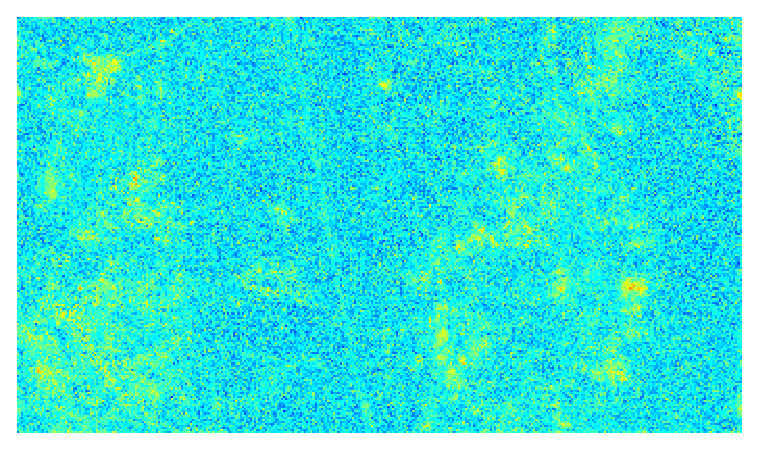
\includegraphics[width=0.3\linewidth]{./figures/chik_expt/MO9/RMSE_MAP_FISTA}};
                \node at (nCenter) [xshift=- 3.5 cm,yshift= 0.0 cm] (nTrue) {\includegraphics[width=0.3\linewidth]{./figures/chikusei_RGB}};
                \node at (nCenter) [xshift=  3.5 cm,yshift= 0.0 cm] (nHybr) {\includegraphics[width=0.3\linewidth]{./figures/chik_expt/MO9/RMSE_MAP_HYBRID}};
                \node at (nFISTA)  [xshift=  0.0 cm,yshift=-3.8 cm] (nCNMF) {\includegraphics[width=0.3\linewidth]{./figures/chik_expt/MO9/RMSE_MAP_CNMF}};
                \node at (nCNMF)   [xshift=- 3.5 cm,yshift= 0.0 cm] (nFUMI) {\includegraphics[width=0.3\linewidth]{./figures/chik_expt/MO9/RMSE_MAP_FUMI}};
                \node at (nCNMF)   [xshift=  3.5 cm,yshift= 0.0 cm] (nHySu) {\includegraphics[width=0.3\linewidth]{./figures/chik_expt/MO9/RMSE_MAP_HySure}};
                \node at (nTrue)   [yshift=- 1.9 cm] {(a) RGB};
                \node at (nFISTA)  [yshift=- 1.9 cm] {(b) \textcolor{orange}{ALGO-FISTA}};
                \node at (nHybr)   [yshift=- 1.9 cm] {(c) \textcolor{orange}{ALGO-HYBRID}};
                \node at (nFUMI)   [yshift=- 1.9 cm] {(d) FUMI};
                \node at (nCNMF)   [yshift=- 1.9 cm] {(e) CNMF};
                \node at (nHySu)   [yshift=- 1.9 cm] {(f) HySure};
                \node at ($(nHybr)!0.5!(nHySu)$) [xshift= 2.7cm]{\includegraphics[width=0.09\linewidth]{./figures/RMSE_bar}} ;
            \end{tikzpicture}
            }
            \caption{RMSE map of Chikusei data set.}
        \end{figure}
    \end{frame}
    \begin{frame}
        \frametitle{Experiments}
        Part 3: \textcolor{orange}{ALGO} vs state-of-the-art algorithms
                on Chikusei data set (a big image with $1000 \times 1000$ pixels).
        \begin{figure}
            \centering
            \resizebox{0.95\linewidth}{!}{
            \begin{tikzpicture}
                \node at (0,0) (nCenter) {};
                \node at (nCenter) [xshift=- 0.0 cm,yshift= 0.0 cm] (nFISTA){\includegraphics[width=0.3\linewidth]{./figures/chik_expt/MO9/SAM_MAP_FISTA}};
                \node at (nCenter) [xshift=- 3.5 cm,yshift= 0.0 cm] (nTrue) {\includegraphics[width=0.3\linewidth]{./figures/chikusei_RGB}};
                \node at (nCenter) [xshift=  3.5 cm,yshift= 0.0 cm] (nHyBr) {\includegraphics[width=0.3\linewidth]{./figures/chik_expt/MO9/SAM_MAP_HYBRID}};
                \node at (nFISTA)  [xshift=  0.0 cm,yshift=-3.8 cm] (nCNMF) {\includegraphics[width=0.3\linewidth]{./figures/chik_expt/MO9/SAM_MAP_CNMF}};
                \node at (nCNMF)   [xshift=- 3.5 cm,yshift= 0.0 cm] (nFUMI) {\includegraphics[width=0.3\linewidth]{./figures/chik_expt/MO9/SAM_MAP_FUMI}};
                \node at (nCNMF)   [xshift=  3.5 cm,yshift= 0.0 cm] (nHySu) {\includegraphics[width=0.3\linewidth]{./figures/chik_expt/MO9/SAM_MAP_HYSURE}};
                \node at (nTrue)   [yshift=- 1.9 cm] {(a) RGB};
                \node at (nFISTA)  [yshift=- 1.9 cm] {(b) \textcolor{orange}{ALGO-FISTA}};
                \node at (nHybr)   [yshift=- 1.9 cm] {(c) \textcolor{orange}{ALGO-HYBRID}};
                \node at (nFUMI)   [yshift=- 1.9 cm] {(d) FUMI};
                \node at (nCNMF)   [yshift=- 1.9 cm] {(e) CNMF};
                \node at (nHySu)   [yshift=- 1.9 cm] {(f) HySure};
                \node at ($(nHybr)!0.5!(nHySu)$) [xshift= 2.7cm]{\includegraphics[width=0.07\linewidth]{./figures/SAM_bar}} ;
            \end{tikzpicture}
            }
            \caption{SAM map of Chikusei data set.}
        \end{figure}
    \end{frame}
    \begin{frame}
        \frametitle{Experiments}
        Part 3: \textcolor{orange}{ALGO} vs state-of-the-art algorithms on
                Chikusei data set (a big image with $1000 \times 1000$ pixels).
        \begin{table}
        \resizebox{0.80\linewidth}{!}{
        \begin{tabular}{|c|l|c|c|c|c|}
        \hline
        SNR (dB)            & \multicolumn{1}{c|}{Method} & RMSE(dB)                              & SAM(deg.)                           & PSNR(dB)                       & Time(sec.)\tnote{3}                      \tabularnewline \hline
        \multirow{3}{*}{40} & FUMI        &                     $-22.58\pm 0.03$    &                     $2.07     \pm 0.01$ &                     $39.61    \pm 0.08$  &                     $2744.03\pm 440.45$  \tabularnewline
                            & CNMF        &                     $-23.77   \pm 0.02$ &                     $2.24     \pm  0$   &                     $44.36    \pm 0.01$  & \cellcolor{red! 10}{$21.19    \pm 1.81$} \tabularnewline
                            & HySure      &                     $-23.35   \pm 0.11$ &                     $2.61     \pm 0.06$ &                     $40.47    \pm 0.25$  &                     $39.3     \pm 6.36$  \tabularnewline
                            & ALGO-FISTA  & \cellcolor{red! 10}{$-25.12\pm 0$}      & \cellcolor{red! 10}{$1.72     \pm 0$}   & \cellcolor{red! 10}{$44.5     \pm 0.03$} &                     $87.23\pm 21.39$     \tabularnewline
                            & ALGO-HYBRID &                    {$-23.08\pm 0.05$}   &                     $2.75     \pm 0.04$ &                     $39.58    \pm 0.11$  &                     $32.5\pm 8.64$       \tabularnewline \hline
        \end{tabular}
        }
        \caption{HSR performance of \textcolor{orange}{ALGO-FISTA} and
                 \textcolor{orange}{ALGO-HYBRID} and FUMI. $N = 9$; $L=1000 \times 1000$; $100$ trials.}
        \end{table}
    \end{frame}
    \begin{frame}
        \frametitle{Experiments}
        %Part 1: Exact BCD vs \textcolor{orange}{ALGO} \\
        %Conclusion: \textcolor{orange}{ALGO} is much better than Exact BCD in
        %            terms of \textbf{runtime} while HSR quality is still
        %            comparable. \\ 
        %\vspace{1cm}
        %Part 2: \textcolor{orange}{ALGO} using different $1^{st}$ order gradient methods. \\
        %Conclusion: \textcolor{orange}{ALGO-FISTA} has better in both HSR
        %            quality and runtime.
        Part 3: \textcolor{orange}{ALGO} vs state-of-the-art algorithms on Chikusei data set. \\
        Conclusion:
        \begin{itemize}
            \item \textcolor{orange}{ALGO-FISTA} has better HSR performance.
            \item big image processing $\rightarrow$ ALGO-HYBRID can be faster than ALGO-FISTA.
            \item CNMF is nevertheless the fastest HSR algorithm.
        \end{itemize}
    \end{frame}
\section{Summary}
    \begin{frame}
        \frametitle{Summary}
        Summary:
        \begin{itemize}
            \item a fast algorithm framework in hyperspectral super-resolution;
            \item \textcolor{orange}{ALGO}: an alternating optimization using Inexact BCD \newline
                  with $1^{st}$ order algorithms;
            \item ALGO requires fewer runtime compared with FUMI and HySure;
            \item illustrate ALGO's capability in handling big data sets.
        \end{itemize}
        \vspace{0.35cm}
        Further discussion:
        \begin{itemize}
            \item the algorithm framework can be extent to similar HSR problem
                  with priori in sparse / smooth abundance $\bm S$;
            \item direct extension to hyperspectral unmixing (HU)
                  \[ \underset{\bm A\in\mathcal A,\bm S\in\mathcal S}{\min} \;
                     \Vert \bm Y - \bm A \bm S \Vert\Fr^2; \]
            \item great potential in problems of MF form.
        \end{itemize}
    \end{frame}
\section{Appendices and References}
\appendix
    \begin{frame}\label{fr:LSMU}
        \frametitle{Appendix: Lee-Seung Multiplicative Update (MU) \hyperlink{fr:SOAs}{\beamerreturnbutton{\tiny return}}}
        \[ \begin{array}{cl}
               \underset{\bm W,\bm H}{\min} &
               \Vert \bm V - \bm W \bm H \Vert\Fr^2 \\
               \text{s.t.} &
               \begin{array}{cc}
                   \bm W \in \R_+^{m \times n}, &
                   \bm H \in \R_+^{n \times \ell}.
               \end{array}
           \end{array} \]
        \centering
        \scalebox{0.90}{
        \begin{minipage}{0.8\linewidth}
        \begin{algorithm}[H]
            \caption*{Lee-Seung MU}
            \begin{algorithmic}[1]
                \Procedure{}{} 
                \newline
                Input: $\bm W_0\geq \bm 0$,
                       $\bm H_0\geq \bm 0$; \;\;\;
                Output: $\bm W$, $\bm H$.
                \smallskip
                \State{$\bm W \gets \bm W_0, \; \bm H \gets \bm H_0$.}
                \For{$i=0,1,2,\cdots$}% until stopping criteria holds}
                    \For{$j=1,2,\cdots$}% or until stopping criteria holds}
                        \State{$\bm H \gets \bm H \cdot \frac{\bm W\Tr \bm V}{\bm W\Tr \bm W \bm H}$.}
                    \EndFor
                    \For{$j=1,2,\cdots$}% or until stopping criteria holds}
                        \State{$\bm W \gets \bm W \cdot \frac{\bm V \bm H\Tr}{\bm W \bm H \bm H\Tr}$.}
                    \EndFor
                    \State{$\bm W$, $\bm H$.}
                \EndFor
            \EndProcedure
            \end{algorithmic}
        \end{algorithm}
        \end{minipage}
        }
    \end{frame}
    \begin{frame}\label{fr:HSR-as-QP}
        \frametitle{Appendix: HSR as QP \hyperlink{fr:HSR-is-QP}{\beamerreturnbutton{\tiny return}}}
        Let $\bm y_1$, $\bm y_2$ and $\bm x$ be the vectorization of
        $\bm Y_1$, $\bm Y_2$ and $\bm X$.
        \begin{eqnarray*}
            &   &
            \underset{\bm X}{\min} \;
            \Vert \bm Y_1 - \bm A_1 \bm X \bm B_1 \Vert\Fr^2 +
            \Vert \bm Y_2 - \bm A_2 \bm X \bm B_2 \Vert\Fr^2 \\
            & = &
            \underset{\bm x}{\min} \;
            \Vert \bm y_1 - \left[ \bm B_1\Tr \otimes \bm A_1 \right] \bm x \Vert_2^2 +
            \Vert \bm y_2 - \left[ \bm B_2\Tr \otimes \bm A_2 \right] \bm x \Vert_2^2 \\
            & = &
            \underset{\bm x}{\min} \;
            \left|\left| \begin{bmatrix} \bm y_1 \\ \bm y_2 \end{bmatrix} -
                         \begin{bmatrix} \bm B_1\Tr \otimes \bm A_1 \\
                                         \bm B_2\Tr \otimes \bm A_2 \end{bmatrix} \bm x\right|\right|_2^2 \\
            & = &
            \underset{\bm x}{\min} \; \; \;
            \bm x\Tr \bm P \bm x + \bm q\Tr \bm x + r
        \end{eqnarray*}
    \end{frame}
    \begin{frame}[allowframebreaks]
        \frametitle{References}
        \bibliographystyle{IEEEbib}
        \footnotesize
        %\setbeamertemplate{bibliography item}[text]
        \bibliography{Bibliography}
    \end{frame}
\end{document}
